\documentclass{article}

\usepackage{fullpage}
\usepackage{amsfonts}
\usepackage{graphicx}
\usepackage{lscape}
\usepackage{endfloat}
\usepackage{color}

\newcommand{\beas}{\begin{eqnarray*}}
\newcommand{\enas}{\end{eqnarray*}}
\newcommand{\bea}{\begin{eqnarray}} \newcommand{\ena}{\end{eqnarray}}
\newcommand{\q}{k} \newcommand{\proof}{ {\bf Proof:} }
\def\squarebox#1{\hbox to #1{\hfill\vbox to #1{\vfill}}}
\newcommand{\qed}{\hfill\hfill\vbox{\hrule\hbox{\vrule\squarebox
{.667em}\vrule}\hrule}\smallskip} \newcommand{\level}{\mbox{$\theta$}}
\newcommand{\vspan}{\mbox{span}} \newcommand{\supp}{\mbox{supp}}
\newcommand{\trace}{\mbox{tr}} \newcommand{\real}{\mathcal Re}
\newcommand{\imag}{\mathcal Im} \newcommand{\diag}{\mbox{diag}}
\newcommand{\offd}{\mbox{off}} \newcommand{\low}{\mbox{low}}
\newcommand{\half}{{\frac{1}{2}}} \newcommand{\quarter}{{\frac{1}{4}}}
\newcommand{\eighth}{{\frac{1}{8}}} \newcommand{\Det}{\mbox{det}}
%\newcommand{\dim}{\mbox{dim}}
\newcommand{\Vscp}{V}
\newcommand{\rank}{\mbox{rank}}
\newcommand{\eig}{\mbox{{\bf eig}}}
\newcommand{\vect}{\mbox{vec}}
\newcommand{\integers}{\mbox{Z}}
\newcommand{\field}{\mathbb{F}}
\newcommand{\reals}{\mathbb{R}}
\newcommand{\complexes}{\mathbb{C}}
\newcommand{\nullspace}{Null}

\newcommand{\Rl}{\mathbb{R}}
\newcommand{\Nl}{\mathbb{N}}
\newcommand{\Ir}{\mathbb{Z}}
\newcommand{\Cx}{\mathbb{C}}
\newcommand{\A}{\mathcal{A}}
\newcommand{\HH}{\mathcal{H}}
\newcommand{\LL}{\mbox{ad}}
\newcommand{\KK}{\mathcal{K}}
\newcommand{\N}{\mathcal{N}}
\newcommand{\Proj}{{\rm Proj}}
\newcommand{\Span}{{\rm span}}
\newcommand{\abs}[1]{\lvert#1\rvert}
\newcommand{\paren}[1]{\left({#1}\right)}
\newcommand{\bparen}[1]{\left\{{#1}\right\}}
\newcommand{\brparen}[1]{\left[{#1}\right]}
\newcommand{\norm}[1]{\left|\left|{#1}\right|\right|}
\newcommand{\inp}[1]{\left<{#1}\right>}
\newcommand{\floor}[1]{\left\lfloor{#1}\right\rfloor}
\newcommand{\ceil}[1]{\left\lceil{#1}\right\rceil}
\newcommand{\ket}[1]{\lvert#1\rangle}

\newtheorem{theorem}{Theorem}[section]
\newtheorem{definition}[theorem]{Definition}
\newtheorem{lemma}[theorem]{Lemma}
\newtheorem{corollary}[theorem]{Corollary}

\newcommand{\Red}{\color{red}}

\title{{\bf Optimized Effective Potential Calculations}}

\author{Ross A. Lippert and N.~A. Modine}

\begin{document}

\maketitle

\section{The Optimized Effective Potential with Finite Temperature}

\subsection{abstract}
The optimized effective potential OEP method provides an additional level
of exactness in electronic structures computations, e.g., the exact
exchange energy can be used.  This extra freedom is likely to be
important in moving density functional methods beyond traditional
approximations such as the local density approximation.  We provide
a new density-matrix-based derivation of the gradient of the Kohn-Sham
energy with respect to the effective potential.  This gradient can be
used to iteratively minimize the energy in order to find the OEP.
Previous work has indicated how this can be done in the zero temperature
limit.  This paper generalizes the previous results to the finite
temperature regime.  Equating our gradient to zero gives a finite-temperature
version of the OEP equation.

\subsection{Introduction}

The Kohn-Sham Density Functional Theory (DFT) \cite{KohnSham:65} has become one of the
most powerful tools for understanding and predicting the properties of materials.  DFT has
been applied to an ever increasing number of different types of systems and
phenomena, and the results have frequently been remarkably useful.  Nevertheless,
the accuracy of the results remains an important issue for many potential
applications of DFT.  The main source of error in DFT calculations is the use
of an approximate expression for the exchange-correlation energy, $E_{XC}$.
Such an approximation is necessary for practical calculations, but improving
the quality of the approximation, and hence, the accuracy of the calculations,
is of great interest.  Conventional variants of DFT, such as LDA and GGA, take
$E_{XC}$ to be an explicit functional of the electronic density.  Since the
noninteracting Kohn-Sham orbitals are implicit functionals of the electronic
density \cite{HohenbergKohn:64},  expressions for $E_{XC}$ that explicitly
depend on the Kohn-Sham orbitals are also consistent with the DFT framework.
An important example of such a functional is the functional used in the exact-exchange
approximation\cite{TalmanShadwick:76, SahniGruenebaumPerdew:82,EngelVosko:93,GorlingLevy:94,
Kotani:95,StadeleMajewskiVoglGorling:97,Gorling99}.  An explicit dependence
on the orbitals allows approximate $E_{XC}$ expressions to capture physical
behaviors of the exact Kohn-Sham $E_{XC}$ that can not be practically incorporated
in an expression that is an explicit function of only the electronic density.  One
example is the absence of self-interaction in the exact Kohn-Sham energy.
Another example is the complex, non-local behavior of the exact exchange energy.

The difficulty in using an $E_{XC}$ expression that is explicitly dependent on
the orbitals is that it is impossible to straightforwardly take the functional
derivative of $E_{XC}$ with respect to the electronic density.  Therefore,
standard self-consistent methods of minimizing the energy with respect to the
density can not be used.  The solution to this problem is provided by the
Optimized Effective Potential (OEP) formalism.  Since the energy is a functional
of the Kohn-Sham orbitals, and the orbitals are solutions of the Kohn-Sham
equation for some local potential, the energy can be viewed as a functional
of the potential.  The OEP is defined to be the potential that minimizes
the energy.  This minimization with respect to the potential is equivalent
to the usual minimization with respect to the density.  Traditionally, the OEP
has been calculated by solving the OEP integral equation, in which the gradient
of the energy with respect to the potential is set to zero \cite{TalmanShadwick:76,
SahniGruenebaumPerdew:82,EngelVosko:93,Kotani:95},
or by directly evaluating and inverting a response function \cite{GorlingLevy:94,
StadeleMajewskiVoglGorling:97,Gorling99}.

Two recent papers have proposed calculation of the OEP by means of an iterative minimization
of the energy \cite{HymanStilesZangwill:00,KummelPerdew:03}.  Hyman, Stiles, and Zangwill
used Lagrange multiplier methods to derive an expression for the gradient of the energy
with respect to the potential and proposed using this gradient to minimize the
energy iteratively.  Kummel and Perdew derived a nearly identical expression and,
although they did not claim that this expression gives the gradient, they noted
that it provides a good update to the potential during an iterative minimization.
In this paper, we present a new derivation of the gradient based on the
density matrix.  Our work goes beyond the previous papers in the following ways:
(1) We believe that our derivation is particularly transparent, and therefore,
it demonstrates that this expression is, in fact, the correct gradient.
(2)  The previous work assumed a negligible electronic temperature.  Since our
derivation is based on the density matrix, it is easily extended to finite
temperatures, where the orbitals are partially occupied.

One of the most exciting recent applications of DFT has been high energy density
physics.  In this application, electronic temperatures that are substantial
compared to the band gaps of typical semiconductors are common.  This makes
the results sensitive to the band gap, which is too small in the standard
versions of DFT. Therefore, the capability of performing calculations with
advanced functionals that have explicit dependence on the orbitals at
non-zero temperature is particularly exciting for high energy density physics
applications.

As an alternative to iterative minimization of the energy using the gradient,
it is possible, in principle, to find the OEP by solving the equation in
which the gradient is set to zero.  Therefore, our work provides the finite
temperature equivalent of the standard OEP equation, giving the correct
necessary condition for local optimality.

In this article, we derive the OEP method in a finite temperature regime
by considering the perturbation of the density matrix resulting from a
perturbed Hamiltonian.
The gradient will reduce to a combination of orbital shifts as one sees
in the zero temperature limit plus some corrections which come from the
finite temperature.  In section \ref{pert_sec}, we begin with a mathematical discussion
of the perturbation theory of analytic functions of Hermitian operators.
After a short review of density functional theory, we apply the results
of section \ref{pert_sec} to the density matrix $\rho$ viewed as a function of
the Kohn-Sham Hamiltonian $H$, and thereby derive a finite temperature OEP
equation in terms of $H$ and $\rho$.   This motivates the subsequent
section, which describes the gradient expression in {\em orbital form}.
We conclude with some computational results demonstrating the accuracy
of the method.

\subsection{The perturbation theory of matrix-analytic functions}

\label{pert_sec}
Let $f(x)$ be an analytic function of $x$ and $f(A)$ be the
extension of $f$ to a matrix-analytic function
(see \cite{HornJohnson.book:91}, chapter 6) on some algebra of
Hermitian operators with a finite (or countable) spectrum.  Thus,
\bea
\label{com_eq}
 [A, f(A)] &=& A f(A) - f(A) A = 0\\
\label{eig_eq}
 f_i &=& f(a_i)
\ena
where the $a_i$ are the eigenvalues of $A$ and the $f_i$ are
the eigenvalues of $f(A)$.

For an unconstrained variation $A \rightarrow A + \delta A$
the variations of (\ref{com_eq}) and (\ref{eig_eq}) are
\bea
\label{dcom_eq}
 [\delta A, f(A)]+[A, \delta f(A)] &=& 0\\
\label{deig_eq}
 \delta f_i &=& f^\prime (a_i) \delta a_i.
\ena
In a basis where $A$ is diagonal
($a_i = A_{ii}, f(a_i) = \left[f(A)\right]_{ii}$),
(\ref{dcom_eq}) and (\ref{deig_eq}) become,
\bea
\label{ddcom_eq}
 (a_i - a_j) \left[\delta f(A)\right]_{ij} &=&  (f(a_i) - f(a_j)) \delta A_{ij}\\
\label{ddeig_eq}
 \delta \left[f(A)\right]_{ii} &=& f^\prime (a_i) \delta A_{ii}.
\ena
Thus (\ref{dcom_eq}) and (\ref{deig_eq})
appear to be sufficient to determine $\delta f(A)$ in terms of $A,\delta A$.

We may, somewhat informally, write the result as one equation
\bea
\label{jac_eq}
 \left[\delta f(A)\right]_{ij} &=& \frac{f(a_i) - f(a_j)}{a_i - a_j} \delta A_{ij}
\ena
where it is understood that we treat
$\frac{f(a_i) - f(a_j)}{a_i - a_j}$
as a {\em divided difference}, taking the limit as $a_i \rightarrow a_j$.

A more rigorous proof of these results can be made in the following theorem,
which also makes clear what happens in the presence of a repeated eigenvalue.
\begin{theorem}
The expansion of $f(A + \delta A) - f(A) = \delta f(A)$
 to first order in $\delta A$ is given by
%The expansion of $f(A + \delta A) - f(A) = \delta f(A) + \delta^2 f(A)$
% to second order in $\delta A$ is given by
\beas
\left[ \delta f(A) \right]_{ij} 
&=& \lim_{\epsilon\rightarrow 0}
     \frac{f(a_i+\epsilon) - f(a_j)}{a_i - a_j+\epsilon}
     \delta A_{ij} %\\
%\left[ \delta^2 f(A) \right]_{ij} 
%&=& 
% \lim_{\epsilon_1,\epsilon_2\rightarrow 0}
% \sum_{p}
%                 \frac{2}{a_i - a_j+\epsilon_1-\epsilon_2}
%		 \left(
%		    \frac{(a_i+\epsilon_1)^k - a_p^k}{a_i - a_p+\epsilon_1}
%		    -\frac{(a_j+\epsilon_2)^k - a_p^k}{a_j - a_p+\epsilon_2}
%		 \right)
%     \delta A_{ip} \delta A_{pj}
\enas
where the matrix elements are taken in an basis in which
$A$ is diagonal.
\end{theorem}
\proof
Since $f$ is analytic, it suffices to prove this theorem for
$f(x) = x^k$ and extend by linearity.

\beas
 \delta f(x) &=& \sum_{m+n=k-1} A^m \delta A A^n %\\
%             &=& \lim_{\epsilon_1,\epsilon_2 \rightarrow 0}
%                      \sum_{m+n=k-1} (A+\epsilon_1 I)^m \delta A (A+\epsilon_2 I)^n  %\\
% \delta^2 f(x) &=& 2 \sum_{l+m+n=k-2} A^l \delta A A^m \delta A A^n\\
%               &=& \lim_{\epsilon_1,\epsilon_2,\epsilon_3 \rightarrow 0}
%                   2 \sum_{l+m+n=k-2} (A+\epsilon_1 I)^l \delta A
%		                    (A+\epsilon_2 I)^m \delta A
%		                    (A+\epsilon_3 I)^n
\enas
in a diagonal basis,
\beas
 \left[\delta f(x)\right]_{ij}
             &=& \sum_{m+n=k-1} a_i^m a_j^n \delta A_{ij}\\
             &=& \sum_{m+n=k-1} \lim_{\epsilon\rightarrow 0} (a_i+\epsilon)^m a_j^n \delta A_{ij}\\
             &=& \lim_{\epsilon\rightarrow 0}
                 \frac{(a_i+\epsilon)^k - a_j^k}{(a_i+\epsilon) - a_j} \delta A_{ij} %\\
%             &=& \lim_{\epsilon_1,\epsilon_2 \rightarrow 0}
%                      \sum_{m+n=k-1} (a_i+\epsilon_1)^m (a_j+\epsilon_2)^n \delta A_{ij}\\
%             &=& \lim_{\epsilon_1,\epsilon_2 \rightarrow 0}
%		      (a_i+\epsilon_1)^{k-1}
%                      \sum_{n=0}^{k-1} \left(\frac{a_j+\epsilon_2}{a_i+\epsilon_1}\right)^{n}
%		      \delta A_{ij}\\
%             &=& \lim_{\epsilon_1,\epsilon_2 \rightarrow 0}
%                      \frac{(a_i+\epsilon_1)^k - (a_j+\epsilon_2)^k}
%			   {(a_i+\epsilon_1) - (a_j+\epsilon_2)}
%                      \delta A_{ij} %\\
% \left[\delta^2 f(x)\right]_{ij}
%               &=& \lim_{\epsilon_1,\epsilon_2,\epsilon_3 \rightarrow 0}
%                   2 \sum_{p,l+m+n=k-2} (a_i+\epsilon_1)^l
%		                    (a_p+\epsilon_2)^m 
%		                    (a_j+\epsilon_3)^n
%		   \delta A_{ip} \delta A_{pj}\\
%               &=& \lim_{\epsilon_1,\epsilon_2,\epsilon_3 \rightarrow 0}
%		 \frac{2}{(a_i+\epsilon_1) - (a_j+\epsilon_3)}
%		 \left(
%                      \frac{(a_i+\epsilon_1)^k - (a_p+\epsilon_2)^k}
%			   {(a_i+\epsilon_1) - (a_p+\epsilon_2)}
%                    - \frac{(a_j+\epsilon_3)^k - (a_p+\epsilon_2)^k}
%			   {(a_j+\epsilon_3) - (a_p+\epsilon_2)}
%		 \right)
%                 \delta A_{ip} \delta A_{pj},
\enas
and the summation is interchanged with the limit.
\qed

Note that one could clearly obtain higher order derivatives in terms of higher order
divided differences via the same approach.  To simplify forthcoming derivations,
we omit $\epsilon$'s and limits,
with the understanding that appropriate limits are to be taken for
divided differences of the form $\frac{f(x) - f(y)}{x-y}$.  We may interpret
(\ref{jac_eq}) as the equation which specifies the action of the {\em
Jacobian}, $\frac{\partial f(A)}{\partial A}$ on an arbitrary
Hermitian operator of the mapping $f$.

\subsubsection{Practical application of the Jacobian}

An $A$-diagonalizing basis might not be a convenient means to compute
the application of the Jacobian to an arbitrary variation.  We
present here a short digression on how such computations can be
carried out iteratively, without diagonalizing $A$.

We will be interested in applications of linear operators to Hermitian
(or anti-Hermitian) matrices.  To avoid some of the confusion entailed
in {\em operators of operators} discussions, we introduce some
notation, which we hope is clarifying.  We denote the application of a
linear operator on a matrix with brackets, $L\left[A\right]$.  In
terms of indices we may write this as $L\left[A\right]_{ij} = \sum_{kl} L_{ijkl} A_{kl}$.
For Hermitian matrices, we write $\left<X,Y\right> =
\trace\{XY\}$, and it is well known that this is a 
non-degenerate inner product on the vector space of Hermitian
matrices.  For a vector subspace of Hermitian matrices, $A$, we let
$A^\perp = \{B: \forall X\in A, \left<X,B\right>=0\}$.

We denote the linear action of a commutator $\LL_{X}\left[Y\right] = -\LL_{Y}\left[X\right] = [X,Y]$.
\begin{lemma}
\label{little_sym_lem}
\beas
\label{ad_transpose_eq}
 \left<X,\LL_Y[Z]\right> = -\left<\LL_{Y}[X],Z\right>.
\enas
\end{lemma}
\proof
Applying the trace identity $\trace\{AB\} = \trace\{BA\}$,
\beas
  \trace\{X (Y Z - Z Y)\}
  &=& \trace\{X Y Z - Y X Z\}\\
  &=& -\trace\{(Y X - X Y) Z\}
\enas
\qed

The {\em centralizer} of $X$ is the set $C_X =\{Y : [X,Y] = 0\}$.
$C_X$ is the nullspace of $\LL_X$.
\begin{lemma}
\label{range_lem}
$C_{X}^\perp$ is the range of $\LL_X$.
\end{lemma}
\proof
For any $Y$ and some $Z \in C_{X}$,
by lemma \ref{little_sym_lem},
$\left<\LL_{X}(Y),Z\right> = -\left<Y,\LL_{X}(Z)\right>=0$,
thus $\mbox{Range}\{\LL_{X}\} \subset C_{X}^\perp$.

From elementary dimension counting,
\beas
\dim\left\{ \mbox{Range}\{ \LL_X \} \right\} 
+ \dim\left\{ \mbox{Null}\{ \LL_X \} \right\}&=&
     \dim\{ C_{X} \} + \dim\{ C_{X}^\perp \} \\
\dim\left\{ \mbox{Range}\{ \LL_X \} \right\} 
+ \dim\left\{ C_X \right\}&=&
     \dim\{ C_{X} \} + \dim\{ C_{X}^\perp \} \\
\dim\left\{ \mbox{Range}\{ \LL_X \} \right\} 
   &=& \dim\{ C_{X}^\perp \} 
\enas
where $\dim\{ C_{X} \} = \dim\{ C_X \}$ obtains the
last line.
\qed

Let $X_{ij} = \frac{f(a_i) - f(a_j)}{a_i - a_j} Y_{ij}$ in an
$A$-diagonalizing basis.
Then according to (\ref{com_eq}) and (\ref{dcom_eq}),
\bea
\label{sparse_com_eq}
  \LL_A[X] &=& \LL_{f(A)}[Y].
\ena
The operator, $\LL_A$, has a non-trivial nullspace.
However, $C_A \subset C_{f(A)}$ implies $\mbox{Range}\{\LL_{f(A)}\}
\subset \mbox{Range}\{\LL_A\}$, by lemma \ref{range_lem}, thus equation 
(\ref{sparse_com_eq}) has a unique solution.

Since we are dealing with a linear space (albeit of matrices),
with a linear operator and an inner product, we can
use a Krylov-based iterative solver to solve (\ref{sparse_com_eq})
(e.g. conjugate gradient or MINRES \cite{minres,GolubVanLoan.book:89})
with some initial guess, $X_0$, yielding
\beas
  X = X_0 + c_1 \LL_A[X_0] +  c_2 \LL_A^2[X_0] + \cdots
\enas
with $X - X_0 \in C_A^\perp$.

By (\ref{deig_eq}), we additionally require $X_{ii} = f^\prime(a_i) Y_{ii}$.
For example, if we take
\beas
  X_0 = \half \left(f^\prime(A) Y + Y f^\prime(A) \right) + X_1,
\enas
where $X_1 \in C_A^{\perp}$ is arbitrary,
then the iterative solution of (\ref{sparse_com_eq}) will be correct,
i.e. $X = \delta f(A)$.  In the remainder of this article we take
$X_1 = 0$.

\subsection{Density functional theory review}

\label{dft_review}
Let $\rho$ be a density matrix (Hermitian),
$K$ be the kinetic energy operator, $V_{I}$ be the ionic (and
external) potential, with $E_{HXC}(\rho)$ the Hartree, exchange, and
correlation energy.  With
$S(P) =  - \trace\{ \rho \log(\rho) + (I-\rho) \log(I-\rho) \}$
as the entropy expression, the variational energy is
\bea
E(\rho) = \trace\{ \rho (K + V_I) \} + E_{HXC}(\rho) - \frac{1}{\beta} S(\rho).
\ena
The unconstrained derivative is 
\bea
\label{uncon_deriv_eq}
\frac{\partial E}{\partial \rho} &=&
 K + V_I + \frac{\partial E_{HXC}}{\partial \rho} +
 \frac{1}{\beta} \log(\rho(I-\rho)^{-1}).
\ena

The Kohn-Sham Hamiltonian is given by $H = K + V_I + \Vscp$ where
$\Vscp$ is the self-consistent potential (to be determined).
In the Kohn-Sham DFT, $\rho$ is the minimizer of
$\trace\{\rho H \} - \frac{1}{\beta} S(\rho)$
with $\trace\{\rho\}=n$, which is equivalent to the conditions,
\bea
\label{rho_eq}
  \rho &=& \frac{1}{1+e^{\beta (H - \mu I)}} = f_\beta(H-\mu I)\\
\label{trace_rho_eq}
  \trace\{\rho\} &=& n
\ena
for some chemical potential $\mu$.
Thus, we can consider $\rho$ to be parametrized by two unknowns
$\Vscp$ and $\mu$ with two relations (\ref{rho_eq}) and (\ref{trace_rho_eq}).
Note: one could absorb $\mu$ into $\Vscp$, but we find it
advantageous to keep it distinct in its role as a Lagrange multiplier.

With $\rho$ satisfying these relations, the energy differential simplifies
\beas
\frac{\partial E}{\partial \rho}
 &=&
 K + V_I + \frac{\partial E_{HXC}}{\partial \rho} +
 \frac{1}{\beta} \log(\rho(I-\rho)^{-1})\\
 &=&
 K + V_I + \frac{\partial E_{HXC}}{\partial \rho} 
 - (H - \mu I)\\
 &=& 
  \frac{\partial E_{HXC}}{\partial \rho} 
 - (\Vscp - \mu I).
\enas
\label{dft_review_sec}

\subsection{Finite temperature OEP with density operators}

From section \ref{dft_review_sec}, the density matrix is
related to the Kohn-Sham Hamiltonian, $H$, by (\ref{rho_eq}) and (\ref{trace_rho_eq}).
Let $\varepsilon_i$ be the eigenvalues of $H$, and let
$\omega_i = f_\beta (\varepsilon_i-\mu)$ be the eigenvalues of $\rho$.
The divided differences can be stably computed with the formula
$$\frac{f_{\beta}(x) - f_{\beta}(y)}{x-y} =
  -\frac{e^{\beta (x+y)/2}}{(1+e^{\beta x})(1+e^{\beta y})}
  \left(\frac{\mbox{sinh}(\beta (x-y)/2)}{(x-y)/2}\right)
$$
where a test for $x=y$ is required for the evaluation of
the last factor.  We note in particular that
$\frac{f_\beta(x)-f_\beta(x)}{x-x} = 
\frac{d}{dx}f_\beta(x) = -\beta f_\beta(x)(1-f_\beta(x))$.

Let $E(\rho)$ be a function of a density matrix, $\rho$.
We can implicitly define $E(H) = E(\rho(H,\mu(H)))$.
Formally varying $E(H)$,
\bea
\label{pre_dE_eq}
 \delta E(H) =
     \trace\left\{
     \frac{\partial E(\rho(H,\mu))}{\partial \rho} \delta \rho
     \right\}.
\ena
in an $H$-diagonalizing basis,
\bea
\label{diag_drho_eq}
 \delta \rho_{ij} = \frac{\omega_i - \omega_j}{\varepsilon_i-\varepsilon_j}
               \left( \delta H_{ij} - \delta \mu \delta_{ij} \right).
\ena
By (\ref{trace_rho_eq}), the trace of $\delta \rho$ vanishes,
\beas
 \delta \mu 
   &=& 
    \frac{\sum_{ij}
      \delta_{ij} \frac{\omega_i - \omega_j}{\varepsilon_i-\varepsilon_j} \delta H_{ij}
    }{\sum_{ij}
      \delta_{ij} \frac{\omega_i - \omega_j}{\varepsilon_i-\varepsilon_j}
    }\\
   &=& \frac{ \trace\{ \rho(I-\rho)\delta H \} }
         { \trace\{ \rho(I-\rho) \} }.
\enas
Thus, in an $H$-diagonalizing basis,
\beas
 \delta E
&=& \sum_{ij}
       \frac{\partial E}{\partial \rho_{ij}} 
       \frac{\omega_i - \omega_j}{\varepsilon_i-\varepsilon_j}
        \left( \delta H_{ij} - \delta \mu \delta_{ij} \right)\\
&=& \sum_{ij}
       \frac{\partial E}{\partial \rho_{ij}} 
       \frac{\omega_i - \omega_j}{\varepsilon_i-\varepsilon_j}
       \left(
       \delta H_{ij}
               -
       \frac{\sum_k \omega_k(1-\omega_k) \delta H_{kk} }
	     {\sum_k \omega_k (1 - \omega_k)}
       \delta_{ij}
       \right)\\
&=&
    \sum_{ij}
    \left(
       \frac{\omega_i - \omega_j}{\varepsilon_i-\varepsilon_j}
       \frac{\partial E}{\partial \rho_{ij}} 
               -
       \delta_{ij}
         \frac{\omega_i(1-\omega_i)}{\sum_k \omega_k (1 - \omega_k)}
    \sum_{pq}  \delta_{pq}
         \frac{\omega_p - \omega_q}{\varepsilon_p-\varepsilon_q}
              \frac{\partial E}{\partial \rho_{pq}}
       \right)       \delta H_{ij}
\enas
and the gradient is therefore
\bea
\label{diag_grad_eq}
 \frac{\partial E}{\partial H_{ij}}
  &=&
       \frac{\omega_i - \omega_j}{\varepsilon_i-\varepsilon_j}
       \frac{\partial E}{\partial \rho_{ij}} 
               -
       \delta_{ij}
         \frac{\omega_i(1-\omega_i)}{\sum_k \omega_k (1 - \omega_k)}
    \sum_{pq}  \delta_{pq}
         \frac{\omega_p - \omega_q}{\varepsilon_p-\varepsilon_q}
              \frac{\partial E}{\partial \rho_{pq}}\\
\label{nodiag_grad_eq}
\frac{\partial E}{\partial H}
  &=& \frac{\Delta \omega}{\Delta \varepsilon}
       \left[\frac{\partial E}{\partial \rho}\right]
       -
       \frac{\rho(I-\rho)}
	    {\trace\{ \rho (I-\rho) \} }
       \trace\left\{\frac{\Delta \omega}{\Delta \varepsilon}
               \left[\frac{\partial E}{\partial \rho}\right]\right\}\\
\label{nodiag_grad_eq2}
  &=& \frac{\Delta \omega}{\Delta \varepsilon}
       \left[\frac{\partial E}{\partial \rho} - 
       \frac{ \trace\left\{\frac{\Delta \omega}{\Delta \varepsilon}
               \left[\frac{\partial E}{\partial \rho}\right]\right\} }
	    { \trace\left\{\frac{\Delta \omega}{\Delta \varepsilon}
              \left[ I \right]\right\} }
	    I
       \right]
\ena
where $\frac{\Delta \omega}{\Delta \varepsilon}\left[\cdot\right]$ stands for
the Jacobian, $\frac{\omega_i - \omega_j}{\varepsilon_i-\varepsilon_j}$,
in a general basis.
$\trace\left\{\frac{\Delta \omega}{\Delta \varepsilon}\left[ I \right]\right\}
= -\beta \trace\{\rho(I-\rho)\}$, though we will keep it as it is in
(\ref{nodiag_grad_eq2}) to make the tracelessness of $\frac{\partial E}{\partial H}$
more manifest.

The application of the Jacobian, to obtain
$\frac{\partial E}{\partial H} = \frac{\Delta \omega}{\Delta \varepsilon}
       \left[\frac{\partial E}{\partial \rho} - 
       \frac{ \trace\left\{\frac{\Delta \omega}{\Delta \varepsilon}
               \left[\frac{\partial E}{\partial \rho}\right]\right\} }
	    { \trace\left\{\frac{\Delta \omega}{\Delta \varepsilon}
              \left[ I \right]\right\} }
	    I
       \right]$,
%$\frac{\Delta \omega}{\Delta \varepsilon}\left[\frac{\partial E}{\partial \rho}\right]$,
can be done by iteratively solving
\bea
\label{DFT_com_eq}
  \left[H,\frac{\partial E}{\partial H} \right]
  = \left[\rho, \frac{\partial E}{\partial \rho}\right]
\ena
with initial guess
\bea
\label{DFT_init_eq}
  \left(\frac{\partial E}{\partial H}\right)_0 &=& 
   -\half \beta \left(
      \rho (I - \rho) \frac{\partial E}{\partial \rho}
    + \frac{\partial E}{\partial \rho} \rho (I - \rho)
  \right)
  + \beta
  \frac{ \trace\left\{\frac{\Delta \omega}{\Delta \varepsilon}
               \left[\frac{\partial E}{\partial \rho}\right]\right\} }
	    { \trace\left\{\frac{\Delta \omega}{\Delta \varepsilon}
              \left[ I \right]\right\} }
   \rho(I - \rho)        .
\ena
Note:
$\lim_{\beta \rightarrow \infty} \beta \rho (I-\rho) \propto \delta(H - \mu I)$,
a delta function on the spectrum of $H$.  Thus in the low temperature limit,
only the eigenvalues of $H$ near $\mu$ contribute to
$\left(\frac{\partial E}{\partial H}\right)_0$.

%It is also worth noting here the asymptotic behavior of the individual
%$\frac{\partial E}{\partial H_{ij}}$ in an $H$-diagonal basis.
%\beas
% \lim_{\omega_i,\omega_j \rightarrow 1}\frac{\partial E}{\partial H_{ij}}&=&0\\
% \lim_{\omega_i,\omega_j \rightarrow 0}\frac{\partial E}{\partial H_{ij}}&=&0,
%\enas
%thus, we see that as $\beta\rightarrow \infty$, the couplings are
%between occupied and unoccupied eigenstates of $H$.  Similarly, we
%see that for finite $\beta$ as $\varepsilon_i,\varepsilon_j \rightarrow \infty$
%the coupling between states $i$ and $j$ vanishes.  These vanishing couplings
%are of great importance when translating these results to an orbital
%representation.

To obtain an OEP gradient, we restrict the
variability of $H$ to $H = H_0 + \Vscp$ where $H_0 = K + V_{I}$ is fixed and $\Vscp$ is a
local operator.  The gradient is then
\bea
\label{dEdV_eq}
 \frac{\partial E}{\partial V(r)} 
     &=& \sum_{ij} \phi_i(r) 
         \frac{\partial E}{\partial H_{ij}} \phi_j^*(r)
\ena
where $\phi_i(r)$ is the eigenvector of $H$ with eigenvalue $\varepsilon_i$
in the position representation.

\label{density_sec}


\subsection{Finite temperature OEP with orbitals}

Instead of representing the density as an operator, it is often
more practical to express $\rho$ in terms of an incomplete basis
of partially occupied orbitals.
Let $\phi_1,\phi_2,\ldots$ be a complete eigenbasis of $H$
sorted non-decreasingly in eigenvalue.  Let $N$ be sufficiently
large that $\omega_{i > N} \sim 0$.  Then we may write truncate
the basis so that
\bea
  \rho = \phi \Omega \phi^\dagger
\ena
where $\phi = \left[ \matrix{ \phi_1 & \phi_2 & \cdots & \phi_N }\right]$,
with $\Lambda$ the diagonal matrix of eigenvalues and
$\Omega$ the diagonal matrix with entries $\omega_1,\ldots,\omega_N$
(i.e. $\Omega = f_\beta(\Lambda - \mu I)$).  Note, $N$ will
usually be much smaller than the number of primitive basis functions, so
$\phi$ will be a rectangular matrix with orthonormal columns,
i.e. $\phi^\dagger \phi = I$ (the $N \times N$ identity)
and $\phi \phi^\dagger$ is the orthogonal projector
onto the span of the $\phi_i$ (and hence commutes with $H$).

Let $\chi$ and $\zeta$ be given by
\beas
\chi &=& \trace\left\{\frac{\Delta \omega}{\Delta \varepsilon}
               \left[\frac{\partial E}{\partial \rho}\right]\right\}
  = \sum_{i\ge 1} -\beta \omega_i (1-\omega_i)
    \phi_i^\dagger\frac{\partial E}{\partial \rho}\phi_i\\
\zeta &=& \trace\left\{\frac{\Delta \omega}{\Delta \varepsilon}\left[I\right]\right\}
  = \sum_{i\ge 1} -\beta \omega_i (1-\omega_i)
\enas
and let $\bar{E}$ and $\bar{J}$ be $N\times N$ matrices given by
\bea
\label{Ebar_def_eq}
%\bar{E}_{ij} &=&
% \phi_i^\dagger \frac{\partial E(\phi \Omega \phi^\dagger)}{\partial \rho} \phi_j
%=
% \frac{\partial E(\phi \Omega \phi^\dagger)}{\partial \rho_{ij}}
\bar{E} =
 \phi^\dagger \frac{\partial E(\phi \Omega \phi^\dagger)}{\partial \rho} \phi
&\quad& \left( \mbox{i.e. }
\bar{E}_{ij} =
 \frac{\partial E(\phi \Omega \phi^\dagger)}{\partial \rho_{ij}}\right)
\\
\label{Jbar_def_eq}
%\bar{J}_{ij} &=&
% \phi_i^\dagger 
%   \frac{\Delta \omega}{\Delta \varepsilon} \left[
%        \frac{\partial E}{\partial \rho}
%  - \frac{\chi}{\zeta} I
%   \right]
%   \phi_j
% =
% \frac{\omega_i - \omega_j}{\varepsilon_i - \varepsilon_j} 
%  \left(\bar{E}_{ij} - \frac{\chi}{\zeta}\delta_{ij}\right).
\bar{J} =
 \phi^\dagger 
   \frac{\Delta \omega}{\Delta \varepsilon} \left[
        \frac{\partial E}{\partial \rho}
  - \frac{\chi}{\zeta} I
   \right]
   \phi
&\quad& \left( \mbox{i.e. }
\bar{J}_{ij} =
 \frac{\omega_i - \omega_j}{\varepsilon_i - \varepsilon_j} 
  \left(\bar{E}_{ij} - \frac{\chi}{\zeta}\delta_{ij}\right)
\right).
\ena
Note that by these definitions,
$\left[\Omega,\bar{E}\right] = \left[\Lambda,\bar{J}\right]$.

Since $\omega_{i>N} \sim 0$, the expressions for $\chi$ and
$\zeta$ can likewise be truncated,
\beas
\chi &=& \sum_{1\le i \le N} -\beta \omega_i (1-\omega_i) \bar{E}_{ii}
      = -\beta \trace\left\{ \Omega(I-\Omega) \bar{E} \right\}\\
\zeta &=& \sum_{1\le i \le N} -\beta \omega_i (1-\omega_i)
      = -\beta \trace\left\{ \Omega(I-\Omega) \right\}\\
\enas
and by (\ref{diag_grad_eq})
\beas
(I-\phi \phi^\dagger)
   \frac{\Delta \omega}{\Delta \varepsilon} \left[
        \frac{\partial E}{\partial \rho} - \frac{\chi}{\zeta} I\right]
(I - \phi \phi^\dagger) = 0,
\enas
thus, we may write (\ref{nodiag_grad_eq}) as
\bea
\label{orb_jacE_eq}
\frac{\partial E}{\partial H} &=&
\frac{\Delta \omega}{\Delta \varepsilon} \left[
    \frac{\partial E}{\partial \rho} - \frac{\chi}{\zeta} I\right] =
  \phi \psi^\dagger + \psi \phi^\dagger,
\ena
where $\phi^\dagger \psi = \psi^\dagger \phi = \half \bar{J}$.
This gives an orbital form of equation (\ref{dEdV_eq}),
\bea
\label{new_oep_eq}
\frac{\partial E}{\partial V(r)}
     &=& \sum_{1\le i\le N} \phi_i(r) \psi_i^*(r)+\psi_i(r) \phi_i^*(r)
\ena
which is similar to the equation derived in numerous sources in the OEP
literature \cite{HymanStilesZangwill:00,KummelPerdew:03}, with a modification of the $\psi$ to
accommodate the finite temperature regime.

It remains to solve for $\psi$, which we may decompose as
$\psi = \psi_{\perp}+\half \phi \bar{J}$,
where $\phi^\dagger \psi_{\perp}=0$.
We can derive an equation for $\psi_{\perp}$,
by multiplying equation (\ref{DFT_com_eq})
on the left by the projector
$I - \phi \phi^\dagger$ (which commutes with $H$) and on the
right by $\phi$ and employing (\ref{orb_jacE_eq}),
\bea
 (I-\phi \phi^\dagger)
 \left[H,\frac{\partial E}{\partial H}\right] \phi 
  &=&
 (I-\phi \phi^\dagger)
 \left[\rho, \frac{\partial E}{\partial \rho}\right]\phi
\\
 (I-\phi \phi^\dagger)
 \left(H \psi - \psi \Lambda\right)
  &=&
 -(I - \phi \phi^\dagger) \frac{\partial E}{\partial \rho} \rho \phi
\\
\label{final_eq}
 H \psi_{\perp} - \psi_{\perp} \Lambda
  &=&
 -(I - \phi \phi^\dagger) \frac{\partial E}{\partial \rho} \phi \Omega.
\ena
The LHS and RHS of (\ref{final_eq}) are orthogonal to $\phi$,
by construction.
Thus we have a well-defined
equation for $\psi_{\perp}$.
%We can solve for $\bar{J}$ in the $\phi$ basis by diagonalization.
An iterative method can thus be used to solve for $\psi_{\perp}$ without any
special initialization beyond $\phi^\dagger \psi_{\perp} = 0$.


\subsection{Computational results}

In order to test the above approach, it was implemented in the orbital representation
within the Socorro electronic
structure software using a plane wave basis set and norm-conserving pseudopotentials.
The conjugate gradient algorithm was used to solve the linear systems involved in the
evaluation of the gradient.  Using this algorithm, the computational cost of solving
the set of linear systems determining $\psi_{\perp}$ is comparable to the cost of
solving the Kohn-Sham eigenproblem for $\phi$.  Therefore, each gradient evaluation
is approximately as computationally expensive as one step of the self-consistency
loop in a standard DFT code.

For traditional approximations to the exact DFT,
such as the Local Density Approximation (LDA) and Generalized Gradient Approximation (GGA),
$E_{HXC}$ is an explicit functional of the electronic density, which is the diagonal of
the density matrix $\rho$ in a position representation.  In this case,
$\frac{\partial E_{HXC}}{\partial \rho}$ has the form of a local potential operator $V_{HXC}$,
and the energy minimum occurs at self-consistency, i.e., when $\Vscp = V_{HXC}$.
In this case, the OEP is the self-consistent potential, and the results of our iterative
minimization approach can be compared directly to well-tested results obtained from
conventional self-consistent methods.  Therefore, we have tested our OEP approach by applying
it to LDA calculations.

Our test system consists of a two atom unit cell of silicon in the diamond structure.  We used a
20 Rydberg plane-wave cutoff and a $2 \times 2 \times 2$ Monkhorst-Pack k-point sampling.
This k-point sampling does not give a converged total energy, but this is not an issue for
the purpose of testing our approach.  Two electronic temperatures were used: (1) Room Temperature
($k_B T = 25.67$ meV), and (2) High Temperature ($k_B T = 1.0$ eV).

\begin{figure}[p]
\includegraphics[height=5in]{Figure_1.ps}
\caption{A comparison of the energy change predicted from the gradient
and the actual energy change observed during a random walk in the
potential.  The filled circles are the calculated values.  The solid
line is a guide to the eye representing perfect agreement.}
\label{fd_test}
\end{figure}

In order to test the correctness of the our gradient, we used the finite difference approach.
During each of a series of steps, the value of $\Vscp$ at each point on a real-space grid was
varied by a small ($o(10^{-4}$)) random perturbation $\Delta V(r)$.  During this random walk, the
energy and the gradient were evaluated at each step.  A linear approximation to the change
in energy during each step is given by
\bea
  \Delta E \approx \int{\frac{\partial E}{\partial V(r)} \Delta V(r) dr}.
\ena
For the small steps taken in this test, we would expect this linear approximation to be accurate if
the gradient is accurate.  Therefore, we can compare this predicted energy change to the actual
energy change observed during the random walk.  The results of this comparison for the high
temperature case are shown in Fig.~\ref{fd_test}.  Since the step direction is random,
this represents a very stringent test of the accuracy of the gradient, and we believe that
the excellent agreement between the predicted and actual energy changes demonstrates
that our approach gives an accurate gradient, even at large electronic temperatures.

\begin{figure}[p]
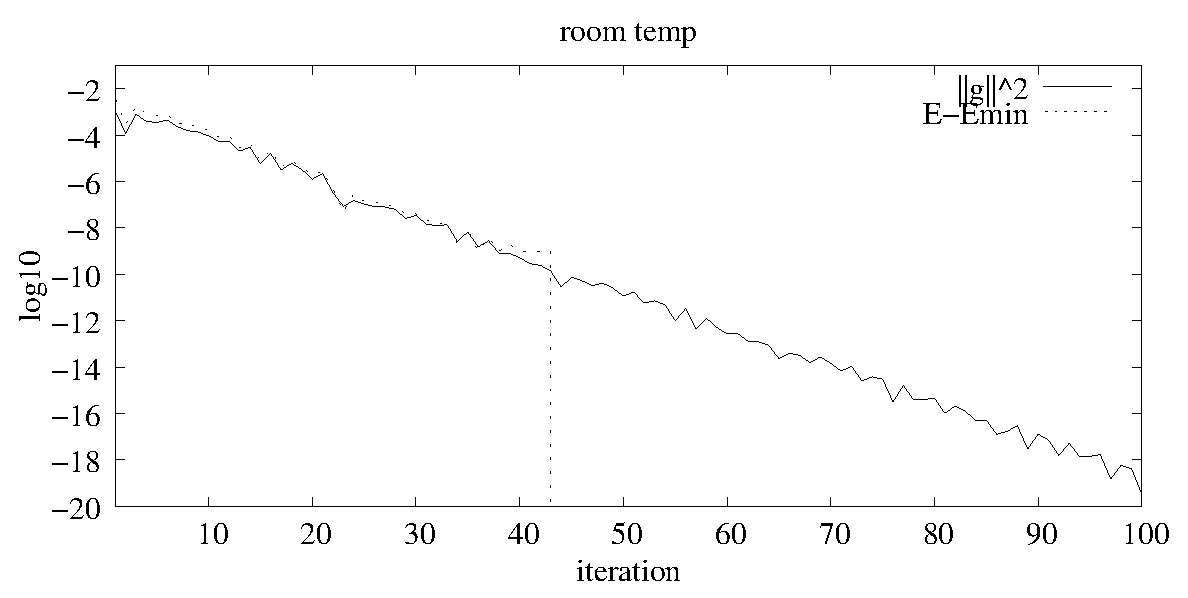
\includegraphics[height=3in]{cvg_room.eps}
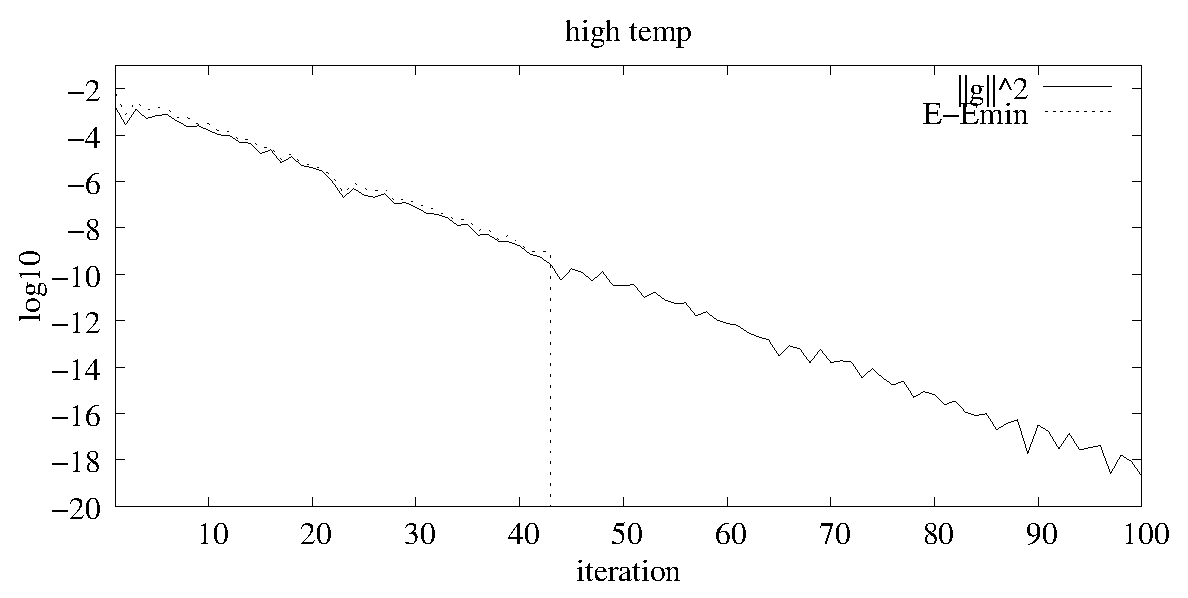
\includegraphics[height=3in]{cvg_1eV.eps}
\caption{The error in the energy, as well as the square-norm of gradient,
during the iterative minimization on a log scale.}
\label{energy_convergence}
\end{figure}

The OEP is found by using the gradient to iteratively minimize the energy.  We implemented this
minimization using Chebyshev acceleration on the fixed point equation
$x_{i+1} = x_i + \tau \nabla f(x_i)$ for some fixed $\tau$ empirically chosen.
The convergence of the energy of our test
system during this process is shown in Fig.~\ref{energy_convergence}.  The errors
in the energy were evaluated by comparing the energies obtained during the iterative minimization
to the result of a highly converged self-consistent calculation.  The convergence demonstrates
that the iterative OEP and self-consistent approaches give the same result, as would be expected
for the LDA energy functional.  The convergence is only weakly dependent on the electronic
temperature.  The asymptotic rate of convergence obtained in the iterative OEP approach is
not as rapid as the highly optimized mixing methods typically used in self-consistent calculations,
but a reasonable accuracy for practical purposes ($10^{-4}$ Ry.) can be obtained easily.

\subsection{Discussion}

We have found and verified an expression for the gradient of the Kohn-Sham energy with
respect to the local potential appearing in the Kohn-Sham Hamiltonian.  Our derivation
based on the density matrix naturally provides a result that is valid at finite temperature.
The cost of evaluating the optimized effective potential using this approach should be
comparable to the cost of a traditional density functional calculation using standard
functionals such as the LDA or GGA, but a greatly extended family of exchange-correlation
functionals that have an explicit dependence on the Kohn-Sham orbitals can be considered.

%\usepackage{fullpage}
%\usepackage{amsfonts}
%
%\newcommand{\beas}{\begin{eqnarray*}}
%\newcommand{\enas}{\end{eqnarray*}}
%\newcommand{\bea}{\begin{eqnarray}} \newcommand{\ena}{\end{eqnarray}}
%\newcommand{\q}{k} \newcommand{\proof}{ {\bf Proof:} }
%\def\squarebox#1{\hbox to #1{\hfill\vbox to #1{\vfill}}}
%\newcommand{\qed}{\hfill\hfill\vbox{\hrule\hbox{\vrule\squarebox
%{.667em}\vrule}\hrule}\smallskip} \newcommand{\level}{\mbox{$\theta$}}
%\newcommand{\vspan}{\mbox{span}} \newcommand{\supp}{\mbox{supp}}
%\newcommand{\trace}{\mbox{tr}} \newcommand{\real}{\mathcal Re}
%\newcommand{\imag}{\mathcal Im} \newcommand{\diag}{\mbox{diag}}
%\newcommand{\offd}{\mbox{off}} \newcommand{\low}{\mbox{low}}
%\newcommand{\half}{{\frac{1}{2}}} \newcommand{\quarter}{{\frac{1}{4}}}
%\newcommand{\eighth}{{\frac{1}{8}}} \newcommand{\Det}{\mbox{det}}
%%\newcommand{\dim}{\mbox{dim}}
%\newcommand{\scp}{\mbox{scp}}
%\newcommand{\rank}{\mbox{rank}}
%\newcommand{\eig}{\mbox{{\bf eig}}}
%\newcommand{\vect}{\mbox{vec}}
%\newcommand{\integers}{\mbox{Z}}
%\newcommand{\field}{\mathbb{F}}
%\newcommand{\reals}{\mathbb{R}}
%\newcommand{\complexes}{\mathbb{C}}
%\newcommand{\nullspace}{Null}
%
%\newcommand{\Rl}{\mathbb{R}}
%\newcommand{\Nl}{\mathbb{N}}
%\newcommand{\Ir}{\mathbb{Z}}
%\newcommand{\Cx}{\mathbb{C}}
%\newcommand{\A}{\mathcal{A}}
%\newcommand{\HH}{\mathcal{H}}
%\newcommand{\LL}{\mbox{ad}}
%\newcommand{\KK}{\mathcal{K}}
%\newcommand{\N}{\mathcal{N}}
%\newcommand{\Proj}{{\rm Proj}}
%\newcommand{\Span}{{\rm span}}
%\newcommand{\abs}[1]{\lvert#1\rvert}
%\newcommand{\paren}[1]{\left({#1}\right)}
%\newcommand{\bparen}[1]{\left\{{#1}\right\}}
%\newcommand{\brparen}[1]{\left[{#1}\right]}
%\newcommand{\norm}[1]{\left|\left|{#1}\right|\right|}
%\newcommand{\inp}[1]{\left<{#1}\right>}
%\newcommand{\floor}[1]{\left\lfloor{#1}\right\rfloor}
%\newcommand{\ceil}[1]{\left\lceil{#1}\right\rceil}
%\newcommand{\ket}[1]{\lvert#1\rangle}
%
%\newtheorem{theorem}{Theorem}[section]
%\newtheorem{definition}[theorem]{Definition}
%\newtheorem{lemma}[theorem]{Lemma}
%\newtheorem{corollary}[theorem]{Corollary}
%

\section{Notes on the choice of OEP cutoff}

It has been noted that the exact exchange OEP optimization
problem seems to suffer from certain pathologies which
can let to either non-uniqueness of the effective potential
at optimality or the equivalence of the calculated OEP density
and energy to that of the corresponding Hartree-Fock quantities.

The argument can be summarized as follows.
Let $P$ be any two-point Hermitian function
(i.e. $P(x_1,x_2) = \bar{P}(x_2,x_1)$).
The total energy functional, in either the Hartree-Fock or exchange-only
KS schemes, is
\beas
E[P] = \trace\bparen{ \paren{-\half \nabla_{x_1}^2 + v_{\mbox{ext}}(x_1) + \half v_J(x_1) }
 P(x_1,x_2) }
 + E_X
\enas
where
$\trace\bparen{ f(x_1,x_2) } = \int f(x,x) dx$ and
\beas
v_J(x) &=& \int \frac{P(x^\prime,x^\prime)}{|x-x^\prime|} dx^\prime\\
E_X &=& - \half \int \frac{P(x_1,x_2) P(x_2,x_1)}{|x_1-x_2|} dx_1 dx_2.
\enas
For the Hartree-Fock method, $E[P]$ is minimized over all
$P$ of the form $P = \sum_{i=1}^{n_e} \phi_i(x_1) \bar{\phi}_i(x_2)$
where $\inp{\phi_i, \phi_j } = \delta_{ij}$.
This local optimality conditions for HF are
$\brparen{P, \hat{H}^{HF}} = 0$, where
\beas
\hat{H}^{HF} = -\half \nabla^2 + v_{\mbox{ext}} + v_J + \hat{K}
\enas
where
\beas
\hat{K} \phi(x) = \int \frac{P(x^\prime,x)}{|x-x^\prime|} \phi(x^\prime) dx^\prime
\enas
For exact exchange-only Kohn-Sham, $E[P]$ is also optimized with the added
condition that the $\phi_i$ are eigenfunctions of
\beas
\hat{H}^{KS} = -\half \nabla^2 + v_{\mbox{ext}} + v_J + v_X
\enas
for some local potential $v_X$, which implies
$\brparen{P, \hat{H}^{KS}} = 0$.  Since this merely restricts
the space of exploration for optimizing $E[P]$, the exact exchange-only
KS solution cannot have a lesser energy than the exact HF solution.

The paper by
Staroverov et al explores seemingly paradoxical results
where, in certain finite bases, it is possible to construct a
$v_X$ such that $\brparen{P, \hat{H}^{KS}} = 0$, i.e.
$P$ satisfies the exact exchange-only KS constraints,
where $P$ is the optimum of the associated Hartree-Fock
problem, and thus
the minimum exact exchange-only KS energy must coincide
with that of HF and $P$ is a solution of the KS problem.

The essence of the argument is the observation that
$\hat{H}^{KS} -  \hat{H}^{HF} = v_X - \hat{K}$, and hence
$\brparen{P, \hat{H}^{KS}} = 0$ if 
$\brparen{ P, v_X } = \brparen{ P, \hat{K} }$.
and $\brparen{ P , \hat{H}^{HF} } = 0$.
If we take $P$ to be the HF minimizer, then
this is not entirely unexpected.
Let $a_\mu(x)$ be real basis functions for the orbitals, thus
$P(x_1,x_2) = \sum_{\mu_1,\mu_2} P_{\mu_1\mu_2} a_{\mu_1}(x_1) a_{\mu_2}(x_2)$,
and $b_{\nu}(x)$ be real basis functions for the potentials,
$v_X = \sum_{\nu} v_{X\nu} b_{\nu}(x)$.  Then, in terms of these
expansions, the relevant products are
\beas
  (v_X P)(x_1,x_2) &=& \sum_{\mu_1 \mu_2 \nu} v_{X\nu} P_{\mu_1\mu_2}
              b_{\nu}(x_1) a_{\mu_1}(x_1) a_{\mu_2}(x_2)\\
  (\hat{K} P)(x_1,x_2) &=&
      \sum_{\mu^\prime \mu_2} P_{\mu^\prime \mu_2}
     \paren{ \int \frac{P(x^\prime,x_1)}{|x_1-x^\prime|} a_{\mu^\prime}(x^\prime) dx^\prime }
     a_{\mu_2}(x_2)\\
 &=&
      \sum_{\mu_1 \mu \mu^\prime \mu_2} P_{\mu^\prime \mu_2}
     \paren{ \int \frac{ P_{\mu \mu_1} a_{\mu}(x^\prime) a_{\mu_1}(x_1) }{|x_1-x^\prime|} a_{\mu^\prime}(x^\prime) dx^\prime }
     a_{\mu_2}(x_2)\\
 &=&
      \sum_{\mu_1 \mu \mu^\prime \mu_2}  P_{\mu \mu_1} P_{\mu^\prime \mu_2}
     \paren{ \int \frac{ a_{\mu}(x^\prime)a_{\mu^\prime}(x^\prime) }{|x_1-x^\prime|} dx^\prime }
     a_{\mu_1}(x_1) a_{\mu_2}(x_2).
\enas
Clearly, we can have $v_X P = \hat{K} P$ by
$b_{\nu(\mu,\mu^\prime)}(x) 
= \int \frac{ a_{\mu}(x^\prime)a_{\mu^\prime}(x^\prime) }{|x-x^\prime|}
   dx^\prime$
and
$v_{X\nu(\mu,\mu^\prime)} P_{\mu_1 \mu_2} = P_{\mu \mu_1} P_{\mu^\prime \mu_2}$
for some appropriate choice of map $\nu(\mu,\mu^\prime)$ between indices
(the possible vanishing of $P_{\mu_1\mu_2}$ is not generic).
Staroverov et al acknowledge that this construction reveals that
for a generic basis of wavefunction, $\{a_\mu\}$, there is at least
one choice of potential basis, $\{ b_{\nu} \}$ such that non-local
effects can be {\em simulated} by an appropriate choice of local potential.
Even for $\{ b_{\nu} \}$ not so pathologically chosen, we might expect
to see some ability to simulate non-local parts of $\hat{K}$ with
a sufficiently large number of basis functions.
It is with the term {\em locality} that we should have an issue.

\subsection{The truly degenerate case}

It is certainly possible that, in a finite wavefunction basis, the optimal
energies given by both the OEP and HF methods coincide.  One very contrived
example is a basis consisting of $n_e$ functions $a_{1},\ldots,a_{n_e}$
where the $a_i(x)$ are the exact orbitals of the Hartree-Fock energy.
In such a basis, no matter what $v_X$ may be, the $P$ corresponding to
the eigenvectors of $\hat{H}^{KS}$ is the identity matrix and is
identical to the Hartree-Fock solution.  Here we see that the
basis, if chosen properly, can ensure that the Kohn-Sham solutions
are arbitrarily close to the Hartree-Fock solutions, independent of the
choice of basis for $v_X$.  Our thesis is that this example is generic.
If the wavefunction basis is sufficiently small, and spans the HF
solution, then the xOEP solution will be forced to resemble the HF solution.
Alternatively, we might consider the wave  function basis fixed and the
potential function basis too big.

\subsection{the basis of $v_X$ is too big}

Consider the plane-wave bases, $a_\mu(x) = e^{i \mu \dot x}$ and
$b_\nu(x) = e^{i \nu \dot x}$ where $\norm{\mu}^2 \le \varepsilon_C$.
Clearly, the eigenvectors of $\hat{H}^{KS}$ are independent of any
potential basis elements with $\norm{\nu}^2 > 4 \varepsilon_C$.
In periodic systems, the number of basis elements for potentials
can be no larger that eight times the number of basis elements for
wavefunctions.  If the wavefunctions have $n$ degrees of freedom,
then the potentials can have, at most, $O(n)$ degrees of freedom.
The construction of Staroverov requires $O(n^2)$ basis functions
for potentials, and thus clearly cannot apply to the case of plane
waves.  The point here is that we should suspect any basis system
which does not have the number of local potential basis elements
proportional to the number of wavefunction basis elements.

There is some reasonably physical reasoning to suspect that the
dimension of potential space should be within a constant (if not
less than or equal to) the dimension of wavefunction space.  If
one considers that ``locality'' of $v_X$ is equivalent to the
demand that $v_X$ commute with the position operator.  The position
operators are matrices of order $|\{a_{\mu}\}|$, in a finite basis.
Hence, the space of operators which commute with the finite basis
position operators can be no more than $|\{a_{\mu}\}|$
dimensional.

For our own plane-wave work, we take $\norm{\nu}^2 \le \varepsilon_C$,
ensuring an equal number of degrees of freedom.  This also has the
effect of removing certain null-vectors of the $v_X$ minimization which
ultimately arise from the ability of the wavefunction basis to represent
the first-order orbital shifts used to compute the OEP gradient.

\subsection{The KS-wavefunctions are not variational}

It is easy to carrying over intutions from previous methods for DFT
which do not apply to OEP calculations.  One of these is that the
energy is variational in the wavefunction basis, i.e. as you add more
elements to the basis, the optimal E value must decrease.  This is
true for traditional DFT and HF, but is not true for xOEP.  Additional basis
functions allow for more accurate $\hat{H}^{KS}$ wavefunctions, of
course, but this need not be accompanied by a decrease in $E[P]$, it
may increase, in fact.  For example, consider a basis which initially
consists of exact HF orbitals.  If the wavefunction basis is extended
by a generic basis function, $E[P]$ can be expected to increase.

In xOEP, $E[P]$ is variational in $v_X$ and, hence, the local potential
basis but not the wavefunction basis.

As an illustration of principle, we outline a hypothetical procedure
to obtain a converged OEP solution.  One fixes a $\{b_\nu\}$ potential
basis and an initial $\{a_\mu\}$ wavefunction basis.  One solves the
finite dimensional OEP problem.  Then one extends the $\{a_\mu\}$
basis with new elements, resolving for $v_X$ with its basis fixed,
until $E[P]$ converges.  The energy can change in either direction
as the wavefunction basis is increased, and this could be a serious
theoretical problem in ascertaining convergence.  One then has an
upper bound on the true OEP energy, variational in $v_X$.  One can
then augment the $\{b_\nu\}$ and begin again.

We suspect that if the wavefunction basis of Staroverov's examples
were extended by even a few basis functions, it would be clear that
their coinciding HF and xOEP solutions were not actually identical.


{\bf **** stop reading here ****}


{\bf Some rambling about cutoffs again}

Suppose I wish to optimize $e(x)$ such that $x = G(y)$ for some $y$.
This is, essentially, the sort of system one solves in an OEP problem.
Clearly, if the matrix
$\frac{\partial G}{\partial y}(y)$ is not full rank (e.g.
more $y$ variables than $x$ variables) such a system can be expected
to have non-unique $y$ solutions.  Applying the usual theory of
constrained optimization (via Lagrange multipliers or what have you)
we obtain the equations for local optimality,
\beas
(\nabla e) \cdot \frac{\partial G}{\partial y} = 0
\enas
which amounts to a number of orthogonality conditions equal to the
number of $y$ variables, expressing the basic idea that
$(\nabla e) \cdot \delta x = 0$ for all
$\delta x = \frac{\partial G}{\partial y} \delta y$ for any $\delta y$.

In OEP problems, $P$ has the role of $x$ and $v_x$ the role of $y$,
while $E[P]$ be the total energy functional and
$G[v_x]$ is the density matrix,
$P = \sum_{i=1}^{n_e} \phi_i \phi_i^\dagger$,
corresponding to the first $n_e$ eigenvectors of
\beas
\hat{H}^{KS} \phi_i = \varepsilon_i \phi_i.
\enas
For a general operator perturbation, $\delta \hat{H}$ of $\hat{H}^{KS}$,
the variation of $P$ is
\beas
\delta P =
 \sum_{i,j} \omega_{ij} \phi_i
 \inp{\phi_i \left|\delta \hat{H}\right| \phi_j}
 \phi_j^\dagger
\enas
where $\omega_{ij}$ are the appropriate divided differences.
and, hence, with some manipulation (and sign errors),
\beas
\frac{\partial E[P]}{\partial P} \bullet \delta P
 &=&
 \frac{\partial E[P]}{\partial P}
 \bullet
 \paren{
 \sum_{i,j} 
 \omega_{ij}\phi_i \inp{\phi_i \left|\delta \hat{H}\right| \phi_j}
 \phi_j^\dagger
 }\\
 &=&
 \hat{H}^{HF}
 \bullet
 \paren{
 \sum_{i,j} 
 \omega_{ij} \phi_i \inp{\phi_i \left|\delta \hat{H}\right| \phi_j}
 \phi_j^\dagger
 }\\
 &=&
 \sum_{i,j}
 \omega_{ij}
 \inp{\phi_j \left|\hat{H}^{HF}\right| \phi_i}
 \inp{\phi_i \left|\delta \hat{H}\right| \phi_j}
 \\
 &=&
 \sum_{i,j}
 \omega_{ij}
 \inp{\phi_j \left|\hat{K} - v_X\right| \phi_i}
 \inp{\phi_i \left|\delta \hat{H}\right| \phi_j}.
\enas
\beas
\min_{v_x} \norm{ \hat{K} - v_X }^2_{\omega}
\enas
where $\norm{ \hat{O} }^2_\omega =
 \sum_{ij} \omega_{ij} 
           \left| \inp{ \phi_i \left| \hat{O} \right| \phi_j} \right|^2$,
$\phi_i$ are the eigenvectors of $\hat{H}^{KS}$, and
$\omega_{ij}$ are appropriate divided differences.

$v_x = \sum_{\nu=1}^{n_\nu} v_\nu b_\nu(x)$
and $\delta \hat{H} = \delta v_X$, we have the optimality
conditions
\beas
 \sum_{i,j}
 \inp{\phi_j \left|\hat{K} - v_X\right| \phi_i}
 \omega_{ij}
 \inp{\phi_i \left|b_\nu \right| \phi_j}
  &=& 0\\
 \sum_{i,j,\nu^\prime}
 v_{\nu^\prime}
 \inp{\phi_j \left|b_{\nu^\prime}\right| \phi_i}
 \omega_{ij}
 \inp{\phi_i \left|b_\nu \right| \phi_j}
 &=&
 \sum_{i,j}
 \inp{\phi_j \left|\hat{K}\right| \phi_i}
 \omega_{ij}
 \inp{\phi_i \left|b_\nu \right| \phi_j}
\enas

If $\delta \hat{H}$ is restricted to a linear combination of
basic perturbations, $\delta \hat{H} = \sum_i c_i \hat{v}_i$

for the lowest $n_e$ eigenvectors $\phi_i$.  This gives a density
$P = \sum_{i=1}^{n_e} \phi_i \phi_i^\dagger$.  The claim is that

{\bf OK, now I talk about bases}

{\bf end of stab}



In infinite dimensions, an operator is considered local when it
commutes with the position operator, $\brparen{ \hat{O}, \hat{x} } = 0$.
For a truncated basis, we believe this is equivalent to the
condition that the matrices with
elements $\inp{ a_{\mu} \left| \hat{x} \right| a_{\mu^\prime }}$
must commute with
$\inp{ a_{\mu} \left| \hat{v}_X \right| a_{\mu^\prime} }$.
This is clearly something violated in the construction above
is likely to violate.

Under this ansatz, one way to automatically obtain a suitable basis,
$b_\nu$ would be to take the eigenvectors $e^\nu_\mu$ of the matrix
with elements $\inp{ a_{\mu} \left| \hat{x} \right| a_{\mu^\prime }}$
and let
$b_{\nu}(x_1,x_2)=
\sum_\mu e^\nu_{\mu_1} e^\nu_{\mu_2} a_{\mu_1}(x_1) a_{\mu_2}(x_2)$,
which looks, at first, like a non-local operator, but is, in fact,
local for the given basis.

In some cases, $b_\nu(x_1,x_2)$ can actually be localized.  For example,
for a truncated plane-wave basis where $a_{\mu}(x) = \exp(i \mu \cdot x)$
where $\mu \in K = \lambda^{-1} \integers^3 \cap \bparen{ \mu : |\mu| \le C }$
for some length scale $\lambda$ and some cutoff $C$,
we can just use the real form of the plane-wave basis:
$b_{\nu}(x) = \bparen{\cos,\sin}(\nu \cdot x)$
where $\nu \in K$, or
$v_X(x) = \sum_{\nu \in K} v_{X \nu} \exp(i \nu \cdot x)$
where $v_{X \nu} = \bar{v}_{X (-\nu)}$.

{\bf I am now going to talk about cutoffs in a kind of rambling way
to try out different ideas and explanations}

In plane-wave computations is to take a cutoff of $2C$, twice the wave
function cutoff, to represent scalar fields.  The reasoning behind this is
that anything beyond $2C$ has a vanishing contribution to any matrix
element.  Since
$\inp{ a_{\mu} \left| \exp(i \nu \cdot x) \right| a_{\mu^\prime }}
 = N \delta_{\nu (\mu - \mu^\prime)}$, the contribution to
the matrix elements from $|\nu| > 2C$ vanishes.  However, we propose
that the basis for $v_X$ be restricted to a cutoff of $C$ for
purposes of practical computation.
The gradient of $E$ with respect to $v_X$ is
\beas
  \sum_i \phi_i(x) \bar{\psi}_i(x) + \bar{\phi}_i(x) \psi_i(x).
\enas
The contributions to various frequencies in the sum formally
range up to $2C$, but near convergence, if the coverged $\phi_i$ are
well-represented by plane-waves with vanishing high frequency
components, the gradient will receive vanishing contributions
at some frequencies between $C$ and $2C$.  As a simplified example,
if the converged $\phi_i$ have zero coefficients for all frequencies
$|\mu|> k$, then the gradient of $v_X$ has exactly zero contribution
at frequencies beyond $C+k$.  This will lead to very ill-conditioned
problems in the minimization.

A more physical way of motivating the more conservative cutoff on
the plane-wave basis for potentials is by considering the effect of
a single plave-wave potential perturbation on the eigensystem,
\beas
\paren{\hat{H} + \epsilon \exp(i \nu \cdot x) } (\phi + \epsilon \psi)
 = (\varepsilon + \epsilon \chi) (\phi + \epsilon \psi)
\enas
for a single $\phi$, presumed to be one of the ground state
eigenvectors of $\hat{H}$ with eigenvalue $\varepsilon$.  We will
presume $\nu$ is large.  The
orbital shift, $\psi$, can be obtained by solving
\beas
 \hat{H} \psi - \varepsilon \psi &=& \paren{ \mu - \exp(i \nu \cdot x) } \phi\\
 \mu &=& \inp{ \phi \left| \exp(i \nu \cdot x) \right| \phi }\\
 \inp{\psi,\phi} &=& 0.
\enas
The presence of $\mu$ in the first equation ensures consistency with
the third equation.  For realistic ground states, we expect $\phi$
to have a spectrum which is concentrated around the origin.  Multiplication
shifts that spectrum from the origin to $\nu$.  For high frequency
spectral components, $\hat{H} \sim -\half \nabla^2$, and we expect
$\psi$ to have significant frequency contributions concentrated around $\nu$.
If $\nu$ is larger than the wave function cutoff, $\psi$ cannot be
adequately represented.  The perturbation has a negligible first
order contribution in the wave function basis, artificially.

Turning this around, we might also say that since $\psi$ physically
represents the coupling of $\phi$ to unoccupied orbitals
through the perturbing potential, if the wave function cutoff is
too small to represent the bulk of these unoccupied orbitals, it
had best not be considered in the potential basis, since its effects
cannot be represented.  Certainly, if you cannot couple represent
the coupling of $0$ frequency to $\nu$, you are in trouble.  This
also suggests that setting the $v_X$ cutoff to the wave function
cutoff is not overly conservative, but is, in fact, minimally
conservative.  One may wish to make the $v_X$ cutoff even
smaller to ensure better representability of the unoccupied couplings.

Setting the $v_X$ cutoff to the wave function cutoff is one way to
circumvent this problem.  Alternatively, one could use an arbitrarily
large $v_X$ cutoff, so long as one represented the $\psi$ functions
to that cutoff.  In most implementations, however, this requires much
modification of existing code to carry out.

%\usepackage{fullpage}
%\usepackage{amsfonts}
%\usepackage{epsfig}
%\usepackage{color}
%
%\newcommand{\beas}{\begin{eqnarray*}}
%\newcommand{\enas}{\end{eqnarray*}}
%\newcommand{\bea}{\begin{eqnarray}} \newcommand{\ena}{\end{eqnarray}}
%\newcommand{\q}{k} \newcommand{\proof}{ {\bf Proof:} }
%\def\squarebox#1{\hbox to #1{\hfill\vbox to #1{\vfill}}}
%\newcommand{\qed}{\hfill\hfill\vbox{\hrule\hbox{\vrule\squarebox
%{.667em}\vrule}\hrule}\smallskip} \newcommand{\level}{\mbox{$\theta$}}
%\newcommand{\vspan}{\mbox{span}} \newcommand{\supp}{\mbox{supp}}
%\newcommand{\trace}{\mbox{tr}} \newcommand{\real}{\mathcal Re}
%\newcommand{\imag}{\mathcal Im} \newcommand{\diag}{\mbox{diag}}
%\newcommand{\offd}{\mbox{off}} \newcommand{\low}{\mbox{low}}
%\newcommand{\half}{{\frac{1}{2}}} \newcommand{\quarter}{{\frac{1}{4}}}
%\newcommand{\eighth}{{\frac{1}{8}}} \newcommand{\Det}{\mbox{det}}
%%\newcommand{\dim}{\mbox{dim}}
%\newcommand{\scp}{\mbox{scp}}
%\newcommand{\rank}{\mbox{rank}}
%\newcommand{\eig}{\mbox{{\bf eig}}}
%\newcommand{\vect}{\mbox{vec}}
%\newcommand{\integers}{\mathbb{Z}}
%\newcommand{\field}{\mathbb{F}}
%\newcommand{\reals}{\mathbb{R}}
%\newcommand{\complexes}{\mathbb{C}}
%\newcommand{\nullspace}{Null}
%
%\newcommand{\Vscp}{V}
%\newcommand{\Rl}{\mathbb{R}}
%\newcommand{\Nl}{\mathbb{N}}
%\newcommand{\Ir}{\mathbb{Z}}
%\newcommand{\Cx}{\mathbb{C}}
%\newcommand{\A}{\mathcal{A}}
%\newcommand{\HH}{\mathcal{H}}
%\newcommand{\LL}{\mbox{ad}}
%\newcommand{\KK}{\mathcal{K}}
%\newcommand{\N}{\mathcal{N}}
%\newcommand{\Proj}{{\rm Proj}}
%\newcommand{\Span}{{\rm span}}
%\newcommand{\abs}[1]{\lvert#1\rvert}
%\newcommand{\floor}[1]{\left\lfloor{#1}\right\rfloor}
%\newcommand{\ceil}[1]{\left\lceil{#1}\right\rceil}
%\newcommand{\ket}[1]{\lvert#1\rangle}
%
%\newtheorem{theorem}{Theorem}[section]
%\newtheorem{definition}[theorem]{Definition}
%\newtheorem{lemma}[theorem]{Lemma}
%\newtheorem{corollary}[theorem]{Corollary}
%

\section{Practical Optimized Effective Potential Calculations}

\subsection{abstract}
During the summer of 2005, these authors attempted to add a production
quality finite temperature OEP capacity to the SOCORRO code.  The OEP
formulation promises to yield more accurate results for density functional
theory.  However, there have been no implementations of the formulation
which address both our scientific goals (finite temperature simulations,
calculation of variational quantities at the optimum) and our
computational goals (utilizing cutoffs and pseudo-potentials,
obtaining good convergence, preconditioning).  We have made substantial
progress towards our goals in both these areas.  We have isolated a number
of computational pitfalls and some new theory concerning variations of the
optimum which we believe have not been noted before.  This document 
reviews and outlines our OEP work and results.

\subsection{Introduction}

{\Red
We really should give a review of what results are currently circulating
about OEP and OEP in finite temperature.  We should say something about
what kinds of systems have been solved and whether or not anyone has
demonstrated the superior performance we expect to see on some interesting
system, like silicon.  What are the practical limitations by currently
reported simulations?  Do we have the only production code ready to do
serious OEP?  Literature searches are dull, but we do need this.  Perhaps
Normand can email that Perdew guy and ask some questions about the state
of the art.
}

\subsection{Review of the OEP formulation}

We have a ``bare'' Hamiltonian $H_0 = K + V_{I}$ representing
the sum of kinetic energy and ionic (or otherwise external) potentials.
The $V_{I}$ operator is theoretically local, but in practice, it is
much more computationally effective to use a non-local pseudo-potential.
We will hence consider $V_{I}$ to be a general operator.

We consider two energy functions
\beas
E_{*} &=& H_0 \bullet \rho + \Vscp \bullet \rho + \frac{1}{\beta}
           \left( \rho \bullet \log \rho + (I-\rho) \bullet\log (I-\rho) \right)\\
E &=& H_0 \bullet \rho + E_{HXC}(\rho) + \frac{1}{\beta}
           \left(\rho\bullet \log\rho +(I-\rho) \bullet\log (I-\rho) \right)\\
  &=& E_{*} + E_{HXC}(\rho) - \Vscp \bullet \rho
\enas
where we adopt the convention $A \bullet B = \trace\{A^H B\}$.
In the OEP formulation,
we consider $\rho$ to be a function of $\Vscp$ defined by the condition
that $I \bullet \rho = n$ and $E_{*}(\rho)$ is minimized with $\Vscp$ fixed.
This is equivalent to the condition that
$\frac{\partial E_{*}}{\partial \rho} = \mu I$, for some
Lagrange multiplier $\mu$.
Thus we may equivalently take
$\rho(\Vscp) = (I + e^{\beta (H_0 + \Vscp - \mu I)})^{-1}$,
where $\mu$ is selected to ensure $I\bullet \rho(\Vscp) = n$.

We then minimize $E(\rho(\Vscp))$ as a function of $\Vscp$.
In translating derivatives in $\rho$ to derivatives in $\Vscp$ we make use of
a {\em chain rule} for functions of Hermitian matrices,
\beas
  \frac{\partial F( f(X) )}{\partial X}
  = \frac{\Delta f}{\Delta x}\left[ 
    \left. \frac{\partial F(Y)}{\partial Y}\right|_{Y = f(X)} \right]
\enas
where the action of $\frac{\Delta f}{\Delta x}\left[\cdot\right]$, in an
$X$ diagonal basis (letting $x_i = x_{ii}$ be the eigenvalues of $X$), is given by
\beas
\left(\frac{\Delta f}{\Delta x}\left[ Z \right]\right)_{ij}
  = \frac{f(x_{i}) - f(x_{j})}{x_{i}-x_{j}} Z_{ij}
\enas
where $ \frac{f(x_{i}) - f(x_{j})}{x_{i}-x_{j}}$ is
a divided difference (i.e. taking derivatives when $x_{i} = x_{j}$).

For the application of interest, our function is
$\omega(\varepsilon) = \frac{1}{1+e^{\beta \varepsilon}}$.
The gradient of $E$ as a function of $\Vscp$ is
\beas
  \frac{\partial E}{\partial \Vscp}
  &=& \frac{\Delta \omega}{\Delta \varepsilon}
      \left[ \frac{\partial E}{\partial \rho} + \nu I \right]\\
  &=& \frac{\Delta \omega}{\Delta \varepsilon}
      \left[ \frac{\partial E_{HXC}}{\partial \rho} - \Vscp + \nu I \right].
\enas
where $\nu$ (actually the derivative of $\mu$) is selected so that 
$I\bullet \frac{\partial E}{\partial \Vscp} = 0$.
Thus, for OEP, where $\Vscp$ is restricted to be a local operator,
and the gradient is
\beas
  \frac{\partial E}{\partial \Vscp}
  &=& \diag\left[\frac{\Delta \omega}{\Delta \varepsilon}
      \left[ \frac{\partial E_{HXC}}{\partial \rho} - \Vscp + \nu I \right]\right],
\enas
where we understand the $\diag$ above to be the diagonal piece of a Hermitian
matrix taken in real space.

At this point, we should comment that when
$\frac{\partial E_{HXC}}{\partial \rho}$ is a local operator, as in the
case of LDA, then one can motivate the so-called {\em self-consistent}
iteration $\Vscp \leftarrow \frac{\partial E_{HXC}}{\partial \rho} + \nu I$,
which should converge nicely as long as 
$\frac{\Delta \omega}{\Delta \varepsilon}$ does not change much.
This is one reason why LDA calculations have never needed 
to think about $\frac{\Delta \omega}{\Delta \varepsilon}$ or a gradient
formulation of LDA.

As an aside, in Hartree-Fock it is the case
that $\frac{\partial E_{HXC}}{\partial \rho}$ is non-local but that
there is no restriction on $\rho$, which can be thought (perversely)
as there being no locality restriction on $\Vscp$, and thus HF is effectively
doing $\Vscp \leftarrow \frac{\partial E_{HXC}}{\partial \rho} + \nu I$
as well.

However, when doing exact exchange
$\frac{\partial E_{HXC}}{\partial \rho}$ is a non-local operator, and
it is not clear how a fixed-point scheme, similar to that of LDA could
be generated.  This leaves us with the gradient search as our best
available approach.

\subsection{OEP Helman-Feynman correction}

One of the surprising results we've obtained is the failure of the
Helman-Feynman theorem in general OEP problems.

The Helman-Feynman theorem is the basis for
doing perturbative analysis of LDA approximations or Hartree-Fock to
obtain variations in the ground state energy
as a result of a varying Hamiltonian.
It says that if the bare Hamiltonian is a linear functon
$H_0(s) = H_0 + s H_1$,
and $E_{min}(s)$ is the minimum of $E$ (as a function of $\Vscp$)
with the given $H_0(s)$, then
\beas
\frac{d E_{min}}{d s} = H_1\bullet \rho(\Vscp)
\enas
where $\Vscp$ is the minimizer at $s=0$,
giving a linearization of the energy which is independent of
any first derivatives of $\Vscp$ at the minimum.
These first order variations of the minimum energy are the basis for
the calculation of a variety of bulk material properties, like conductivity,
the dielectric constant, as well as stress and strain.
This is
what one would generally expect from an arbitrary
function of the form $f(s) = \min_{x} F(s,x)$, a short sketch of
why being,
\beas
 \frac{\partial}{\partial x} F(x,s) &=& 0\\
 \frac{d}{d s} F(x(s),s) &=& \frac{\partial}{\partial x} F(x(s),s) \frac{dx(s)}{ds} + \frac{\partial}{\partial s} F(x(s),s)\\
                        &=& 0 + \frac{\partial}{\partial s} F(x(s),s).
\enas
However, our problem is analogous to
\beas
 \frac{\partial}{\partial y} F(x(y,s),s) &=&
 \frac{\partial}{\partial x} F(x(y,s),s) \frac{\partial x}{\partial y} = 0\\
 \frac{d}{d s} F(x(y(s),s),s) &=&
 \frac{\partial}{\partial x} F(x(y,s),s)
 \left(\frac{\partial x}{\partial y} \frac{dy(s)}{ds} + 
       \frac{\partial x}{\partial s}\right)
 + \frac{\partial}{\partial s} F(x(y(s),s),s)\\
                              &=&
 \frac{\partial}{\partial x} F(x(y,s),s)
       \frac{\partial x}{\partial s}
 + \frac{\partial}{\partial s} F(x(y(s),s),s),
\enas
and it is this 
$\frac{\partial}{\partial x} F(x(y,s),s)
       \frac{\partial x}{\partial s}$
term, which comes from the fact that the relation between $x$ and $y$ is
dependent on $s$,  that we must account for.

For the OEP formulation,
\beas
\frac{d}{ds} E &=&
         \frac{\partial E}{\partial H} \bullet H_1+
          \frac{\partial E}{\partial s}\\
 &=&
      \left( \frac{\partial E_{HXC}}{\partial \rho} - \Vscp + \mu I \right)
      \bullet       \frac{\Delta \omega}{\Delta \varepsilon}
      \left[H_1\right]+ \trace\{\rho H_1\}\\
 &=&
      \frac{\Delta \omega}{\Delta \varepsilon}
      \left[ \frac{\partial E_{HXC}}{\partial \rho} - \Vscp + \mu I \right]
      \bullet H_1+ \trace\{\rho H_1\}
\enas
The second term vanishes if
\begin{itemize}
\item $H_1$ is local (since the local part of 
$\frac{\Delta \omega}{\Delta \varepsilon}
      \left[ \frac{\partial E_{HXC}}{\partial \rho} - \Vscp + \mu I \right]$
vanishes)
\item LDA: $\frac{\partial E_{HXC}}{\partial \rho}$ is local
(since $\frac{\partial E_{HXC}}{\partial \rho} - \Vscp + \mu I$ vanishes)
\item Hartree-Fock: $\Vscp$ is not restricted to be local
(since $\frac{\partial E_{HXC}}{\partial \rho} - \Vscp + \mu I$ vanishes)
\end{itemize}
Thus, this correction is not present in the previous methods of
LDA and Hartree-Fock.  Corrections to higher order derivatives are
thus also expected to appear in an OEP problem with non-local
$\frac{\partial E_{HXC}}{\partial \rho}$.
{\Red Does the first bullet mean that the HF correction disappears
when you are doing forces?}

\subsubsection{Higher derivatives}

Although we have avoided any considerations of higher derivatives of
the relation between $rho$ and $\Vscp$, it might be important to
list their forms.

Higher order variations on $f(X)$ can be given by divided differences
which generalize the first variation formula
\beas
\left(\frac{\partial f(X)}{\partial X}\left[Z\right]\right)_{ij}
 &=&
  \frac{f(x_{i}) - f(x_{j})}{x_{i}-x_{j}} Z_{ij}\\
\left(\frac{\partial^2 f(X)}{\partial X^2}\left[Z^{(1)},Z^{(2)}\right]\right)_{ij}
 &=&
  \sum_k \frac{
  \frac{f(x_{i}) - f(x_{k})}{x_{i}-x_{k}}
  -\frac{f(x_{j}) - f(x_{k})}{x_{j}-x_{k}}
  }
       {x_{i}-x_{j}}
 \left(Z^{(1)}_{ik} Z^{(2)}_{kj}+Z^{(2)}_{ik} Z^{(1)}_{kj}\right)\\
\left(\frac{\partial^n f(X)}{\partial X^n}\left[Z^{(1)},\ldots,Z^{(n)}\right]\right)_{ij}
 &=&
 \sum_{k_1,\ldots,k_{n-1}} f[x_{i},x_{k_1},\ldots,x_{k_{n-1}}
                                 x_{j}]
 \sum_{\sigma \in S_n} 
  Z^{(\sigma_1)}_{ik_1} Z^{(\sigma_2)}_{k_1k_2} \cdots Z^{(\sigma_{n-1})}_{k_{n-2}k_{n-1}} Z^{(\sigma_n)}_{k_{n-1}j}
\enas

\subsection{A review of the application of
$\frac{\Delta \omega}{\Delta \varepsilon}\left[\cdot\right]$}

A full diagonalization of $H = H_0 + \Vscp$ is computationally impractical
for large basis sets.  We review here how the OEP gradient can be found
by solving for 
$\frac{\Delta \omega}{\Delta \varepsilon}\left[Z \right]$ 
(for $Z$ a Hermitian operators) iteratively
on a set of orbitals $\phi = \pmatrix{\phi_1 & \cdots & \phi_N}$ which
are the lowest $N$ eigenvectors of $H$ with
eigenvalues $\varepsilon_i$ and occupations $\omega_i$ (we assuming
$\omega_i \sim 0$ for $i>N$).

We will generalize slightly, to the computation of $\frac{\Delta
\omega}{\Delta \varepsilon}\left[Z + \nu I \right]$, where $\nu$ is
chosen so that $\trace\{\frac{\Delta \omega}{\Delta
\varepsilon}\left[Z + \nu I \right]\} = t$ (in the case where there is
no trace constraint, $\nu = 0$.
Let $\bar{E}$ and $\bar{J}$ be $N\times N$ matrices given by
\beas
\bar{E} &=&
 \phi^\dagger Z \phi
\\
\bar{J} &=&
 \phi^\dagger 
   \frac{\Delta \omega}{\Delta \varepsilon} \left[
        Z
  + \nu I
   \right]
   \phi
 =\left[
 \frac{\omega_i - \omega_j}{\varepsilon_i - \varepsilon_j} 
  \right] \circ
  \left(\bar{E} + \nu I \right),
\enas
where
$\left[\frac{\omega_i - \omega_j}{\varepsilon_i - \varepsilon_j}\right]$
is the $N\times N$ matrix of divided differences, $\circ$ denotes
elementwise multiplication and $\nu$ is chosen such that
$\trace\{\bar{J}\}=t$.
Let $\psi_{\perp}$ satisfy $\phi^\dagger \psi_{\perp} = 0$ and
\bea
\label{psi_perp_eq}
H \psi_{\perp} - \psi_{\perp} \Lambda
  &=&
 -(I - \phi \phi^\dagger) Z \phi \Omega,
\ena
where $\Lambda,\Omega$ are diagonal matrices with entries
$\varepsilon_i,\omega_i$ respectively.
Then
\beas
\frac{\Delta \omega}{\Delta \epsilon}\left[ Z + \nu I\right]
      = \psi_{\perp} + \frac{1}{2} \phi \bar{J}.
\enas

We see that we can compute
$\frac{\Delta \omega}{\Delta \epsilon}\left[ Z + \nu I \right]$
from products of the form $Z \phi$.  However, this does require an
iterative solution to (\ref{psi_perp_eq}).  It is customary to
allow fairly loose tolerances for the underlying eigenproblem when far from
convergence.  Thus, $\phi$ may be substantially different from
the true lowest eigenvalues of $H$ and $[\phi \phi^\dagger, H]$
may not be small.  In that case, we can do additional projection,
\beas
(I - \phi \phi^\dagger) H \psi_{\perp} - \psi_{\perp} \Lambda
  &=&
 -(I - \phi \phi^\dagger) Z \phi \Omega,
\enas
to ensure that we take a principle submatrix of the
$\left[H,\cdot\right]$ operator on the left hand side, and thus
a well-posed problem.  Even so, if an iterative solution method
requiring positive definiteness is used, poorly converged $\phi$ can
lead to a principle submatrix which is not positive definite.

Generally, we have found that we require our tolerances for the
eigenvectors, $\phi$, to be a bit higher than those required for
self-consistent LDA.

\subsection{OEP gradients in the non-interacting free metal}

In order to obtain some insight into the relation of the various
OEP derived quantities we have been exploring, we can take a look at a
system of plane waves.  In fact, we will simplify things further by
considering non-interacting plane waves.

Since the system is non-interacting, the $E_{HXC}$ term vanishes
and $\Vscp = 0$ is optimal.  The gradient is
\beas
  \frac{\partial E}{\partial \Vscp} = 
\diag\left(\frac{\Delta \omega}{\Delta \varepsilon}\left[ 0 \right]\right)
\enas
which can be varied by $\Vscp \rightarrow 0 + \delta V$ to obtain
the variation of the gradient,
\beas
\delta \frac{\partial E}{\partial \Vscp} &=& 
\diag\left(\frac{\Delta \omega}{\Delta \varepsilon}\left[ -\delta V \right]\right)
+\diag\left(\left(\delta \frac{\Delta \omega}{\Delta \varepsilon}\right)\left[ 0 \right]\right)
\\
&=&
-\diag\left(\frac{\Delta \omega}{\Delta \varepsilon}\left[ \delta V \right]\right)
\enas
Thus we see that the Hessian is given by the action of the Jacobian
restricted to local operators $\delta V$.  There being no possibility
of confusion, we will drop the $\delta$ and use $V$ for a variation of
the (vanishing) optimum effective potential.

Let us suppose that we have a discrete set of wave numbers $K \subset
\reals^3$, which we will use to represent the occupied orbitals of an
idealized system.  In this case, the density operator is
\beas
\rho(\bar{x},\bar{x}^\prime)
= \sum_{\bar{k} \in K} |\bar{k}><\bar{k}|
= \frac{1}{N} \sum_{\bar{k}\in K} e^{-i\bar{k} \cdot(\bar{x}-\bar{x}^\prime)}.
\enas
with $\rho(\bar{x},\bar{x}) = n_e/N$ where $n_e = |K|$ is the number of
electrons and $N$ is the unit volume.

%It can be shown that for any zero temperature system, the local part
%of the Jacobian acting on a local potential $V(\bar{x})$ is given by
%\beas
%   V(\bar{x}) &\rightarrow&
%    2 \sum_{\bar{k} \in K, \bar{k}^\prime \notin K}
%    |\bar{k}><\bar{k}| V |\bar{k}^\prime><\bar{k}^\prime|\\
%  &=&
% 2 \int d\bar{x}^\prime 
%  \left(\rho(\bar{x},\bar{x})\delta(\bar{x}-\bar{x}^\prime) -
%        |\rho(\bar{x},\bar{x}^\prime)|^2\right) V(\bar{x}^\prime)\\
%   &=& 2 \rho(\bar{x},\bar{x}) V(\bar{x}) - 
%        2 \int d\bar{x}^\prime |\rho(\bar{x},\bar{x}^\prime)|^2
%         V(\bar{x}^\prime)
%\enas
%which, for plane waves, becomes,
%\beas
% V(\bar{x}) &\rightarrow&
%   \frac{2 n_e}{N} V(\bar{x}) - 
%   \frac{2}{N^2} \sum_{\bar{k},\bar{k}^\prime\in K}
%        \int d\bar{x}^\prime
%e^{-i (\bar{k}-\bar{k}^\prime)\cdot(\bar{x}-\bar{x}^\prime) }
%         V(\bar{x}^\prime).
%\enas
%The eigenmodes for this action are likewise planewaves,
%$e^{-i \bar{\alpha} \cdot \bar{x}}$ with eigenvalues
%$\frac{2}{N} \left( n_e - n_{\bar{\alpha}} \right)$
%where $n_{\bar{\alpha}} = |\{ (\bar{k},\bar{k}^\prime) \in K^2 | \bar{k} - \bar{k}^\prime = \bar{\alpha}\}|$,
%i.e. the number of occupied orbitals whose wave numbers differ by
%$\bar{\alpha}$.
%Note: $\bar{\alpha} = 0$ is the only zero mode, corresponding to constant
%shifts in the local operators.
%Thus, the effective condition number of the Jacobian restricted to
%local operators is
%$\frac{\max\{n_e - n_{\bar{\alpha}}\}}{\min\{n_e - n_{\bar{\alpha}}\}}$
%where the minimum is taken over $\bar{\alpha}\ne 0$.

%If $K = \{ \bar{k} \in \integers^3 | ||\bar{k}|| \le k_{\max}\}$, then we
%would expect the condition number to be $\sim \frac{2}{3} k_{\max}
%\sim \sqrt[3]{\frac{2}{9} n_e}$.

We can carry out a general derivation for planewaves in finite
temperature, by taking $D_{\bar{k}\bar{k}^\prime}(\beta) =
 \frac{\omega(\varepsilon_{\bar{k}})-\omega(\varepsilon_{\bar{k}^\prime})}
      {\varepsilon_{\bar{k}}-\varepsilon_{\bar{k}^\prime}}$
and thus the localized Jacobian is given by
\beas
  V(\bar{x}) &\rightarrow&
    \sum_{\bar{k},\bar{k}^\prime} D_{\bar{k}\bar{k}^\prime}(\beta)
    |\bar{k}><\bar{k}| V |\bar{k}^\prime><\bar{k}^\prime|\\
  &=&
  \sum_{\bar{k}\bar{k}^\prime}
  e^{-i\bar{k}\cdot \bar{x}}  e^{i\bar{k}^\prime \cdot \bar{x}}
  D_{\bar{k}\bar{k}^\prime}(\beta)
  \int d^3 \bar{x}^\prime
  e^{ i\bar{k}\cdot \bar{x}^\prime}  e^{-i\bar{k}^\prime \cdot \bar{x}^\prime}
  V(\bar{x}^\prime)\\
  &=&
  \sum_{\bar{k}\bar{k}^\prime}
  D_{\bar{k}\bar{k}^\prime}(\beta)
  \int d^3 \bar{x}^\prime
  e^{-i (\bar{k}-\bar{k}^\prime) \cdot (\bar{x}-\bar{x}^\prime)}
  V(\bar{x}^\prime)\\
  &=&
  \sum_{\bar{\alpha}}
  d_{\bar{\alpha}}(\beta)
  \int d^3 \bar{x}^\prime
  e^{-i \bar{\alpha} \cdot (\bar{x}-\bar{x}^\prime)}
  V(\bar{x}^\prime)\\
  &=&
  \sum_{\bar{\alpha}}
  d_{\bar{\alpha}}(\beta)
  |\bar{\alpha}><\bar{\alpha}|
  V
\enas
where $d_{\bar{\alpha}}(\beta) =
  \sum_{\bar{k}-\bar{k}^\prime = \bar{\alpha}}
  D_{\bar{k}\bar{k}^\prime}(\beta)$.  We notes that if
$\int d^3 \bar{x} V(\bar{x})$ vanishes, then so does the 
integral of the RHS, thus $\nu = 0$, and the sum over $\bar{\alpha}$
can be restricted to $\bar{\alpha} \ne \bar{0}$.

We may consider a more specific metallic case where
the possible states are all $\reals^3$ with
\beas
\varepsilon_{\bar{k}} &=& ||\bar{k}||^2\\
\omega(\bar{k}) &=& \frac{1}{1 + e^{\beta(||\bar{k}||^2 - \mu)}}
\enas
where $\mu$ is selected by
$
\int \frac{4 \pi k^2 dk}{1 + e^{\beta(k^2 - \mu)}} = n,
$
for some constant $n$.

Passing from sums to integrals we find (taking $\alpha = ||\bar{\alpha}||$),
\beas
d_{\alpha}(\beta) &=&
\sum_{\bar{k}} D_{(\bar{k}+\half\bar{\alpha})(\bar{k}-\half\bar{\alpha})}\\
&=&
\int \frac{
\omega(\bar{k}+\half \bar{\alpha}) - \omega(\bar{k}-\half \bar{\alpha})
}{
 2 \bar{k} \cdot \bar{\alpha}
}
d^3\bar{k}\\
d_{\alpha}(\beta) &=&
\int \frac{
\frac{1}{1+e^{\beta( (x+\half\alpha)^2 + y^2 + z^2 - \mu)}}
- \frac{1}{1+e^{\beta( (x-\half\alpha)^2 + y^2 + z^2 - \mu)}}
}{
 2 x \alpha
}
dx dy dz\\
&=&
\int_{r \in \reals_+} \int_{x\in \reals}
\pi r \frac{
\frac{1}{1+e^{\beta( (x+\half\alpha)^2 + r^2 - \mu)}}
- \frac{1}{1+e^{\beta( (x-\half\alpha)^2 + r^2 - \mu)}}
}{
 x \alpha
}
dx dr\\
&=&
\int_{x\in \reals}
\pi \frac{
\left.
\log
\frac{1+e^{\beta( (x-\half\alpha)^2 + r^2 - \mu)}}
     {1+e^{\beta( (x+\half\alpha)^2 + r^2 - \mu)}}
\right|_{r=0}^\infty
}{
 2 \beta x \alpha
}
dx\\
&=&
\int_{x\in \reals}
\pi \frac{
\log
\frac{e^{\beta( (x-\half\alpha)^2 - \mu)}}
     {e^{\beta( (x+\half\alpha)^2 - \mu)}}
-
\log
\frac{1+e^{\beta( (x-\half\alpha)^2 - \mu)}}
     {1+e^{\beta( (x+\half\alpha)^2 - \mu)}}
}{
 2 \beta x \alpha
}
dx\\
&=&
\int_{x\in \reals}
\frac{\pi}{2x\alpha} \frac{1}{\beta}
\log
\frac{e^{-\beta( (x+\half\alpha)^2 - \mu)}+1}
     {e^{-\beta( (x-\half\alpha)^2 - \mu)}+1}
dx.
\enas
Taking the limit as $\beta \rightarrow \infty$, noting that
$\lim_{\beta \rightarrow \infty} \frac{1}{\beta} \log(e^{\beta c}+1)
=\max\{c,0\}$ for all $c$,
\beas
d_{\alpha}(\infty)
 &=&
\int_{x\in \reals}
\frac{\pi}{2 x \alpha}
\left(\max\left\{\mu - (x+\half\alpha)^2,0\right\}
-\max\left\{\mu - (x-\half\alpha)^2,0\right\}\right)
dx\\
 &=&
 \int_{x=\half \alpha - \sqrt{\mu}}^{\half \alpha + \sqrt{\mu}}
\frac{\pi}{x \alpha}
\left((x-\half\alpha)^2-\mu\right)
dx\\
 &=&
\int_{x=\half \alpha - \sqrt{\mu}}^{\half \alpha + \sqrt{\mu}}
\pi
\left(\frac{x}{\alpha} -1 + \frac{\frac{1}{4} \alpha^2-\mu}{x \alpha}\right)
dx\\
 &=&
\left.
\pi
\left(\frac{x^2}{2\alpha}-x + \frac{\frac{1}{4} \alpha^2-\mu}{\alpha}\log|x|\right)
\right|_{x=\half \alpha - \sqrt{\mu}}^{\half \alpha + \sqrt{\mu}}\\
 &=&
-\pi
\left(\sqrt{\mu} - \frac{\frac{1}{4} \alpha^2-\mu}{\alpha}
\log\frac{\half \alpha + \sqrt{\mu}}{\left|\half \alpha - \sqrt{\mu}\right|}
\right).
\enas

We now note some of the features of $d_\alpha(\infty)$.  It is continuous
everywhere, taking the value $-\pi\sqrt{\mu}$ at $\alpha = 2\sqrt{\mu}$.
It is differentiable for all $\alpha \ne 2\sqrt{\mu}$
(where it is infinite),
which is associated with the Friedel oscillations in metals.

For large $\alpha$,
\beas
d_\alpha(\infty)
 &=&
-\pi
\left(\sqrt{\mu} - \frac{\frac{1}{4} \alpha^2-\mu}{\alpha}
\log\frac{1+\frac{2\sqrt{\mu}}{\alpha}}{1-\frac{2\sqrt{\mu}}{\alpha}}\right)
\\
 &=&
-\pi
\left(\sqrt{\mu} - \left(\frac{1}{4} \alpha-\frac{\mu}{\alpha}\right)
2 \left(\frac{2\sqrt{\mu}}{\alpha} + \frac{1}{3}\left(\frac{2\sqrt{\mu}}{\alpha}\right)^3 + \cdots\right)\right)
\\
&=&
-\pi
\left(\frac{4 \mu^{3/2}}{\alpha^2}
-\left(\frac{1}{2} \alpha-\frac{2\mu}{\alpha}\right)
\left(\frac{1}{3}\left(\frac{2\sqrt{\mu}}{\alpha}\right)^3 + \cdots\right)
\right)
\\
&\sim&
-\pi
\frac{8 \mu^{3/2}}{3 \alpha^2}.
\enas

For small $\alpha$,
\beas
d_\alpha(\infty)
 &=&
-\pi
\left(\sqrt{\mu} - \frac{\frac{1}{4} \alpha^2-\mu}{\alpha}
\log\frac{1+\frac{\alpha}{2\sqrt{\mu}}}{1-\frac{\alpha}2\sqrt{\mu}}\right)
\\
&=&
-\pi
\left(\sqrt{\mu} - \left(\frac{1}{4} \alpha-\frac{\mu}{\alpha}\right)
2 \left(\frac{\alpha}{2\sqrt{\mu}} + \frac{1}{3}\left(\frac{\alpha}{2\sqrt{\mu}}\right)^3 + \cdots\right)\right)
\\
&\sim&
-\pi
\left(2\sqrt{\mu}
-\frac{\alpha^2}{6\sqrt{\mu}}
\right).
\enas

A bit of empirical curve fitting and screwing around then shows that
\beas
C \sqrt{\mu} \le
d_{\alpha}(\infty) \cdot
\left(
\frac{1}{1+\frac{\alpha^2}{\mu}}
+\frac{3\alpha^2}{4 \mu}\right) \le 2 C \sqrt{\mu}
\enas
for some C, which implies that
\beas
\frac{1}{1-\frac{\nabla^2}{\mu}}
-\frac{3\nabla^2}{4 \mu}
\quad\mbox{or}\quad
1 - \frac{3}{4\mu} \nabla^2
\enas
should be a good preconditioner in the low temperature regime.

We have used the $1 - \frac{3}{4 \mu} \nabla^2$ preconditioner in our
OEP implementation.  It seems to be doing a good job even on non-metallic
silicon.


\subsection{Accelerating convergence}

Since line minimization is expensive and the Hessian in this
case is difficult to apply, we explore a {\em fixed step}
approach such as Richardson iteration.

The basic relaxation step is of the form
\beas
  x_{i+1} = x_i - \gamma g_i,
\enas
where $g_i = \nabla f(x_i)$, which linearizes to
\beas
  x_{i+1} = x_i + \gamma (b - A x_i).
\enas
The iteration on the error $e_i = x_i - x_*$ is given by
\beas
  e_{i+1} &=& (I - \gamma A) e_i\\
  e_{i} &=& (I - \gamma A)^i e_0
\enas
from which we see that $e_i \rightarrow 0$ only if
$-1 \le 1 - \gamma \lambda \le 1$ for all eigenvalues $\lambda$ of $A$.

If the eigenvalues of $A$ occur in $(0,1)$ then convergence
occurs when $\gamma \le 2$ and $\gamma = 2$ is the largest convergent
step size.
In practice, we do not start with the spectrum of $A$ in $(0,1)$,
but we scale all gradients by an empirically determined factor to place
the eigenvalues of $A$ between $(0,1)$ in a more-or-less centered
fashion.

With $\gamma = 2$, if $\lambda_{\min} = \epsilon$ or
$\lambda_{\max} = 1-\epsilon$,
the error in the extreme modes will be $|1 - 2 \epsilon|^i$.
Thus convergence is eventually dominated
by the value of $\kappa = \frac{1}{\epsilon}$,
which is approximately equal to the condition number of $A$.

One technique which works well when good estimates of the Hessian
norm and condition number are available is {\em Chebyshev acceleration}.
One considers a Chebyshev polynomial, $T_i$, affinely
translated so that $(-1,1)\rightarrow (\epsilon,1)$ where the
eigenvalues of the Hessian occur in $(\epsilon,1)$.
The goal is to have $e_i =
\frac{1}{T_i(\beta)} T_i(\beta - \alpha A) e_0$ where $\alpha =
\frac{2}{1-\epsilon}$ and $\beta = \frac{1+\epsilon}{1-\epsilon}$.
The Chebyshev polynomials, given by
\beas
  T_0(y) &=& 1\\
  T_1(y) &=& y\\
  T_{i+1}(y) &=& 2 y T_{i}(y) - T_{i-1}(y).
\enas
The error will decrease roughly as
$\frac{1}{T_i(\beta)}
\sim \left(\frac{1-\sqrt{\epsilon}}{1+\sqrt{\epsilon}}\right)^{-i}$
with a need for periodic resets to correct non-linearities
(which should be reasonable to perform after $2/\sqrt{\epsilon}$ steps).

The recurrences for Chebyshev polynomials can be re-arranged a bit to
give
\beas
\tau_0 &=& 1\\
\tau_1 &=& 1\\
\tau_{i+1} &=& 2 \tau_i - \beta \tau_{i-1}\\
x_1 &=& x_0 - \alpha g_0\\
x_{i+1} &=& x_{i} +
\frac{1}{\tau_{i+1}}\left(\tau_{i-1} \beta (x_i-x_{i-1}) -2 \tau_i \alpha g_i\right)
\enas
and thus we need only keep around a {\em velocity} vector
$x_{i} - x_{i-1}$ and mix it with the gradient to obtain the
update.

With the preconditioner in place, it is reasonable to assume that
Hessian norms and condition numbers are fairly insensitive to problem
size.  We have observed that the same pair of parameters achieve
nearly the same convergence on $2$ atom, $8$ atom, and $64$ atom
silicon, supporting this intuition.  This also suggests that one
might use smaller systems to estimate the optimal convergence
parameters for larger ones.

\subsection{Potential cut-offs}

{\Red This argument is something of a handwave, but I think I only
ever had a handwave argument for it. It works though.}

Let us consider the case where we have used a planewave basis with
some cutoff $||\bar{k}|| < k_W$ and fully diagonalized $H = H_0 + \Vscp$
into a complete eigenbasis $\phi_1,\ldots,\phi_N$ (where $N$ is the
dimension of the planewave basis).  Let us also assume that we have
likewise represented the local operator, $\Vscp$,
in a planewave basis with a cutoff of $k_V$.

We consider the case where
$\Vscp = \Vscp_* + \epsilon e^{i \bar{\alpha} \cdot \bar{x}}$,
where $\Vscp_*$ is the optimal and $v$ is small.  Then the gradient at
$\Vscp$ is
\beas
  \frac{\partial E}{\partial V}
  &=& \diag\left( \frac{\Delta \omega}{\Delta \varepsilon} \left[
       \frac{\partial E_{HXC}(\rho)}{\partial \rho}
       - \Vscp_* - \epsilon e^{i \bar{\alpha}\cdot \bar{x}}
       + (\nu_*+v \gamma) I
       \right]\right)
  = -\epsilon\diag\left( \frac{\Delta \omega}{\Delta \varepsilon} \left[
        e^{i \bar{\alpha}\cdot \bar{x}} - \gamma I
       \right]\right)
\enas
where $\gamma$ is chosen to make $\frac{\partial E}{\partial V}$
traceless.  In terms of the complete eigenbasis,
\bea
\label{deltar_eq}
  \frac{\Delta \omega}{\Delta \varepsilon}
       \left[
        e^{i \bar{\alpha}\cdot \bar{x}}
       \right]
  &=& - \sum_{ij}
    \left(\frac{\omega_i - \omega_j}{\varepsilon_i-\varepsilon_j}\right)
    \left(\phi_i^{\dagger} e^{i \bar{\alpha} \cdot \bar{x}} \phi_j\right)
    \phi_i \phi_j^{\dagger},
\ena
from which we see a vanishing gradient for $||\bar{\alpha}|| > 2 k_W$.
This is to be expected, however, since the coupling between $\Vscp$ and
$\rho$ in $E_*$ is $\Vscp \bullet \rho$ and
$e^{i \bar{\alpha} \cdot \bar{x}} \bullet \rho$ identically vanishes
when $||\bar{\alpha}|| > 2 k_W$.  One way to look at this is that high
frequency modes of $\Vscp$ have no effect on $\rho$ in the presence of
cutoffs, and thus, no effect on the energy $E$.  If we started the
minimization from
$\Vscp=\Vscp_* + \epsilon e^{i \bar{\alpha} \cdot \bar{x}}$, we could not
expect to see $\epsilon$ decrease.

However, this is not enough.  We have observed that with $\Vscp$ cutoff
at $2 k_W$ the convergence of the gradient search is very sub-linear.

In fact, any first order perturbation to $\Vscp_*$ which gives a
second order gradient could not be expected to decrease rapidly
(i.e. linearly) in a gradient-based minimization.  Such perturbations
are then null vectors of the objective function $E(\rho(\Vscp))$.

Consider that in order for a term in (\ref{deltar_eq}) to contribute
significantly to the sum, at least one of $\phi_i$ or $\phi_j$ must
have $\omega_i,\omega_j$ non-vanishing, i.e. be {\em partially
occupied}.  In a typical calculation, the partially occupied states
have planewave components which become vanishingly small for
$||\bar{k}|| > k_0$ with $k_0$ independent of $k_{W}$ so long as
$k_{W}$ is picked to be well enough above $k_0$ (an extreme case is
the free non-interacting metal in which $k_{0}$ is minimal and
independent of $k_W$ for $k_W > k_0$).  Thus if $||\bar{\alpha}|| >
k_{W}+k_{0}$ the first order contribution to $\rho$ will be likewise
small and ill-conditioning of the optimization results.

This ill-conditioning is entirely non-physical, coming from the choice
of $k_W$.  If we consider the effect of increasing $k_{W}$, $k_{0}$
would change negligibly, and thus $k_W + k_0$ would increase and more
$\bar{\alpha}$'s would be able to significantly contribute
(\ref{deltar_eq}).  In non-OEP formulations, the criterion for $k_W$
is to provide a good representation of the partially occupied
orbitals.  However, the OEP gradient couples unoccupied and partially
occupied orbitals, and this coupling can only be represented
faithfully so long as the unoccupied orbitals can be represented
faithfully.

We have used a more stringent cutoff for $\Vscp$ therefore, taking it
to be $k_W$ instead of the customary $2 k_W$.  We have found, with
experiments on silicon, that the number of correctly converged digits
in the resulting energies did not change.  This is to be expected,
since a tiny contribution to the gradient indicates a tiny
contribution to the overall energy.


%\bibliographystyle{abbrv}
%\bibliography{/home/r1/lippert/REF/ref}

\begin{thebibliography}{1}

\bibitem{KohnSham:65}
W.~L. Kohn and L.~J. Sham, Phys. Rev. {\bf 140}, A1133 (1965).

\bibitem{HohenbergKohn:64}
P. Hohenberg and W. Kohn, Phys. Rev. {\bf 136}, B864 (1964).

\bibitem{TalmanShadwick:76}
J.~D. Talman and W.~F. Shadwick, Phys. Rev. A {\bf 14}, 36 (1976).

\bibitem{SahniGruenebaumPerdew:82}
V. Sahni, J. Gruenebaum, and J. P. Perdew, Phys. Rev. B {\bf 26}, 4371 (1982).

\bibitem{EngelVosko:93}  E. Engel and S.~H. Vosko, Phys. Rev. A {\bf 47}, 2800 (1993);
Phys. Rev. B {\bf 50}, 10498 (1994).

\bibitem{GorlingLevy:94}
A. G\"{o}rling and M. Levy, Phys. Rev. A {\bf 50}, 196 (1994).

\bibitem{Kotani:95}
T. Kotani, Phys. Rev. Lett. {\bf 74}, 2989 (1995).

\bibitem{StadeleMajewskiVoglGorling:97}
M. St\"{a}dele, J.~A. Majewski, P. Vogl, and A. G\"{o}rling, Phys. Rev. Lett. {\bf 79}, 2089 (1997);
M. St\"{a}dele, M. Moukara, J.~A. Majewski, P. Vogl, and A. G\"{o}rling, Phys. Rev. B {\bf 59},
10031 (1999).

\bibitem{Gorling99}
A. G\"{o}rling, Phys. Rev. Lett. {\bf 83}, 5459 (1999).

\bibitem{HymanStilesZangwill:00}
R.~Hyman, M.~Stiles, , and A.~Zangwill.
\newblock A gradient search method for orbital-dependent charge-density and
  current density functional calculations.
\newblock {\em Phys. Rev. B}, 62(23):15521--15526, 2000.

\bibitem{KummelPerdew:03}
S.~K\"{u}mmel and J.~P. Perdew.
\newblock Simple iterative construction of the optimized effective potential
  for orbital functionals, including exact exchange.
\newblock {\em Phys. Rev. Letters}, 90(4):043004, 2003.

\bibitem{HornJohnson.book:91}
R.~A. Horn and C.~R. Johnson.
\newblock {\em Topics in Matrix analysis}.
\newblock Cambridge University Press, Cambridge, 1991.

\bibitem{minres}
C.~C. Paige and M.~A. Saunders.
\newblock Solution of sparse indefinite systems of linear equations.
\newblock {\em {SIAM} J. Numer. Anal.}, 12:617--629, 1975.

\bibitem{GolubVanLoan.book:89}
G.~H. Golub and C.~F.~V. Loan.
\newblock {\em Matrix Computations}.
\newblock Johns Hopkins University Press, Baltimore, Maryland, 2d edition,
  1989.

\end{thebibliography}

\end{document}

